\chapterimage{orange_cat.jpg}
\chapter{Some category theory}

\section{Motivation}

\section{Categories and functors}
\begin{exr}
A category in which each morphism is an isomorphism is called a groupoid. (This notion is not important in what we will discuss. The point of this exercise is to give you some practice with categories, by relating them to an object you know well.)
\begin{enumerate}[label=(\alph*)]
\item A perverse definition of a \textit{group} is: a groupoid with one object. Make sense of this.
\item Describe a groupoid that is not a group.
\end{enumerate}
\end{exr}
\begin{proof}\ 
\begin{enumerate}[label=(\alph*)]
\item Consider a groupoid $\cala$ with only one object $A$. Then we can interpret the composition of morphism as a binary product and $id_A$ as the identity $e$. In this way $\cala$ can be interpreted as a group.
\item We can recall the definition of fundamental groupoid $\Pi(M)$, where objects are points $x\in M$ and morphism $Mor(x,y)$. Or we can artificially construct a category illustrated by the following diagram.
\begin{figure}[h]
\centering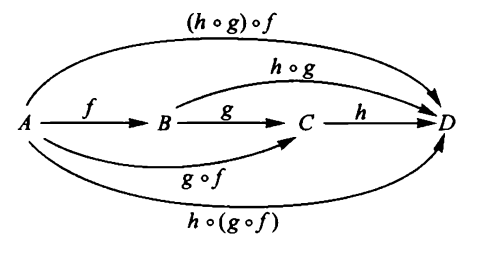
\includegraphics[scale=0.5]{Groupoid}
\caption{A nontrivial groupoid}
\end{figure}
\end{enumerate}
\end{proof}

\begin{exr}
If $A$ is an object in a category $\calc$, show that the invertible elements of $\mor(A, A)$ form a group (called the automorphism group of $A$, denoted $\text{Aut}(A)$). What are the automorphism groups of the objects in $\mathit{Sets}$ and $\mathit{Vec}_k$. Show that two isomorphic objects have the same automorphism groups.
\end{exr}
\begin{proof}
For $\text{Sets}$, the the automorphism group of an object $A$ is the group of permutation of the set $A$. For $\text{Vec}_k$, the automorphism group of $V$ is $\text{GL}_k(V)$. 

Consider two isomorphic objects $A,B$ in $\calc$, $\exists f\in \mor(A,B), g\in\mor(B,A)$ s.t. $f\circ g=id_A$ and $g\circ f=id_B$. Consider $h\in\text{Aut}(B)$, then $g\circ h\circ f\in \text{Aut}(A)$ with inverse $g\circ h^{-1} \circ f$. We can check that it is a isomorphism of groups. It has an inverse $[\forall j\in Aut(A),j\longmapsto g\circ j\circ f]$.
\end{proof}

\begin{exr}
Let $(\cdot)^{\vee\vee} : \text{f.d.Vec}_k \lrta \text{f.d.Vec}_k$ be the double dual functor from the category of finite-dimensional vector spaces over k to itself. Show that $(\cdot)^{\vee\vee}$ is naturally isomorphic to the identity functor on $\text{f.d.Vec}_k$. (Without the finite- dimensionality hypothesis, we only get a natural transformation of functors from $\text{id}$ to $(\cdot)^{\vee\vee}$.)
\end{exr}
\begin{proof}
Recall the definition of natural transformation,
\begin{center}
\begin{tikzcd}
F(A) \arrow[d, "m_A"'] \arrow[r, "F(f)"] & F(A') \arrow[d, "m_{A'}"] \\
G(A) \arrow[r, "G(f)"'] & G(A'),
\end{tikzcd}
\end{center}
In the special case where $F=(\cdot)^{\vee\vee}$ and $G=id$
\begin{center}
\begin{tikzcd}
A \arrow[r, "f"]\arrow[d, "m_A"'] & A' \arrow[d, "m_{A'}"]\\
A^{\vee\vee}  \arrow[r, "f^{\vee\vee}"'] & A'^{\vee\vee}
\end{tikzcd}
\end{center}
$$
\begin{aligned}
m_A:&\ A\lrta A^{\vee\vee}\\
&  v\longmapsto v^{\vee\vee}:=[\forall u^\vee\in A^\vee, u^\vee\longmapsto u^\vee(v)],\\
f^{\vee\vee}: &\ A^{\vee\vee}\lrta A'^{\vee\vee}\\
& w^{**}\longmapsto w^{**}\circ f^{\vee}:=[\forall u'^\vee\in A'^\vee: u'^\vee\longmapsto w^{**}(u'^\vee\circ f)], 
\end{aligned}
$$
where we use $u^{**}$ to denote general element in $A^{\vee\vee}$ distinguishing it from the element generated by $v\longmapsto v^{\vee\vee}$. Then we can 
check compatibility (the diagram commutes)
$m_{A'}\circ f\overset{?}{=}f^{\vee\vee}\circ m_A$
$$
\begin{aligned}
\Llrta&\forall u\in A, m_{A'}\circ f (u)\overset{?}{=}f^{\vee\vee}\circ m_A (u)\\
\Llrta&\forall u\in A,\ f(u)^{\vee\vee}= m_{A'}\circ f (u)\overset{?}{=}f^{\vee\vee}\circ u^{\vee\vee}=u^{\vee\vee}f^\vee\\
\Llrta & \forall u\in A, \forall w'^{\vee}\in A'^{\vee},\  f(u)^{\vee\vee}(w'^\vee)\overset{?}{=}u^{\vee\vee}f^{\vee}(w'^\vee)\\
\Llrta & \forall u\in A, \forall w'^{\vee}\in A'^{\vee},\  w'^\vee(f(u))\overset{\checkmark}{=}w'^\vee\circ f(u).
\end{aligned}
$$
The above abstract nonsense are always true for $k$-vector spaces whether it is finite dimension or not, hence it is always a natural transformation. But when we restrict to finite dimensional vector spaces. 
$v^{\vee\vee}=0\Lrta $ it maps all $u^\vee$ to zero, hence $u^\vee(v)=0,\forall u^\vee\Lrta v=0$. $m_A$ is always injective. When $V$ is finite dimension, $\dim(V^{**})\geq \dims(V^*)\geq \dims(V)$, and we get equality when it is finite dimensional. In this case $m_A$ is an isomorphisms. 
\end{proof}
\begin{exr}
$\mathcal{V}$ is the category of finite dimensional vector spaces of the form $k^n$.
Show that $\mathcal{V}\lrta \text{f.d.Vec}_k$ gives an equivalence of categories, by describing an ``inverse'' functor.
\end{exr}
\begin{proof}
The functor $F:\mathcal{V}\lrta \text{f.d.Vec}_k$ is just the inclusion as a sub category. Assume we can simultaneously choose a basis for each vector space. It has an quasi-inverse functor $G$, such that for $n$-dimensional vector space $V$, $ m_A:V\lrta k^n$, $\{e_{V,i}\}\longmapsto $ \{the standard basis of $k^n$\}.

\begin{center}
\begin{tikzcd}
F\circ G(V) \arrow[d, "m_V"'] \arrow[r, "FG(f)"] & F\circ G(V') \arrow[d, "m_{V'}"] \\
id_{Vec}(V) \arrow[r, "id(f)"'] & id_{vec}(V'),
\end{tikzcd}
\end{center}

$$
\begin{aligned}
F\circ G &(V)=k^n\\
m_V: &k^n\lrta V \\ &(k_1,...,k_n)\longmapsto \sum_i k_i e^{V}_i,
\end{aligned}
$$
and for $f:V\lrta V'$ a $k$-linear morphism, $FG(f):k^n\lrta k^m$ is the linear transformation encoded by the matrix $M^f$ such that $f(e^{V}_j)=\sum_i(M^f)_{ij}e^{V'}_i$. It is now quite easy to check the diagram commutes and $m_V$ is an isomorphism.
\end{proof}

\begin{theorem}
We say that a covariant functor $F:\cala\lrta \calb$ is \textbf{essentially surjective} if every object $B$ in $\calb$ is isomorphic to $F(A)$ for some object $A$ in $\cala$. $F$ is an equivalence of categories iff $F$ is fully faithful and essentially surjective.
\end{theorem}
\begin{proof}
$\Lrta$: Assume $F$ is an equivalence of categories with a quasi-inverse $G$. $F\circ G\cong id_\calb$ and $G\circ F\cong id_\cala$. 
\begin{center}
\begin{tikzcd}
F\circ G(B) \arrow[d, "\mu_B"'] \arrow[r, "FG(f)"] & F\circ G(B') \arrow[d, "\mu_{B'}"] \\
id_{\calb}(B) \arrow[r, "id(f)"'] & id_{\calb}(B'),
\end{tikzcd}
\begin{tikzcd}
G\circ F(A) \arrow[d, "\eta_A"'] \arrow[r, "GF(f)"] & G\circ F(A') \arrow[d, "\eta_{A'}"] \\
id_{\cala}(A) \arrow[r, "id(f)"'] & id_{\cala}(A'),
\end{tikzcd}
\end{center}
each is a natural isomorphism. $f\mu_B=\mu_{B'}FG(f)$.

\underline{$F$ is essentially surjective}: It is clear because every $B\in \calb$ we have $B\cong F(G(B))$, where $G(B)$ is an object in $\cala$. Similarly, we have $G$ is essentially surjective.

\underline{$F$ is full}: $\mu_B$ is isomorphism, which means it has an inverse. Then we composite its inverse from right. We get $f=\mu_{B'}\circ FG(f)\circ \mu_B^{-1}$. Similarly we have $FG(f)=\mu_{B'}^{-1}\circ f\circ \mu_{B}$. Then the map $f\longmapsto FG(f)$ is a bijection between $\mor_{\calb}(B,B')$ and $\mor_{\calb}(FG(B),FG(B'))$. In particular, $f\longmapsto FG(f)$ is surjective, hence the map $G(f)\longmapsto FG(f)$. $\tilde{F}:\mor_\cala(G(B),G(B'))\lrta \mor_\calb(FG(B),FG(B'))$ is surjective but by the fact that $G$ is essentially surjective, ( every object in $\cala$ is isomorphic to some $G(B)$). We know $F:\mor_\cala(A,A')\lrta \mor_\calb(F(A),F(A'))$ is surjective.

\underline{$F$ is faithful}: Similarly we have the map: $f\longmapsto GF(f)$ is an isomorphism between  $\mor_{\cala}(A,A')$ and $\mor_{\cala}(GF(A),GF(A'))$. In particular,$f\longmapsto GF(f)$ is injective, hence the map $f\longmapsto F(f)$ is injective (monic) as a map from $\mor_\cala(A,A')$ to $\mor_\calb(F(A),F(A'))$.

$\Llta$: This time, we know $F$ is essentially surjective fully faithful. 

\underline{Construction of quasi-inverse}:
Since $F$ is essentially surjective, for each object $B$ in $\calb$, there is an object $A$ s.t. $F_{ob}(A)\cong B$ (Assume the axiom of choice, we can simultaneously choose such a representative $A$ for each $B$). We denote the isomorphism $j:B\lrta F(A)$ and $j':B'\lrta F(A')$. Then we define the map $G_{ob}:\text{obj}(\calb)\lrta \text{obj}(\cala)$, $G_{ob}(B)=A$. For each morphism $g\in \mor_\calb(B,B')\cong\mor_{\calb}(F(A),F(A'))$, where the second isomorphism is induced by the isomorphisms $F(A)\cong B$ and $F(A')\cong B'$. We can write the corresponding morphism as $j'\circ g\circ j^{-1}$.

Because $F$ is fully faithful there is a unique morphism $f\in \mor_\cala(A,A')$ so that $j'\circ g\circ j^{-1}=F_{mor}(f)$. ($G_{mor}(g)=F_{mor}^{-1}(j'\circ g \circ j^{-1})$) Then we define $G_{mor}:\mor_\calb(B,B')\lrta \mor_{\cala}(A,A')$, $g\longmapsto f$ as above. (Again, by the axiom of choice, we can assign an $f$ for $g\in \mor_{\calb}(B,B')$ simultaneously for all $g,B,B'$). These datum combine together to form a functor $G$. 

 Then it remains to check $FG\cong id_\calb$ and $GF\cong id_\cala$.
\begin{center}
 \begin{tikzcd}
B \arrow[d, "\mu_B"'] \arrow[r, "g"] & B' \arrow[d, "\mu_{B'}"] \\
F\circ G(B) \arrow[r, "FG(g)"'] & F\circ G(B'),
\end{tikzcd}
\end{center}

\underline{$FG\cong id_\calb$}: Because $FG(B)=F(A)\cong B$ by the definition of functor $G$, $\mu_B$ is just the isomorphism $j:B\lrta F(A)$. Also $FG(g)=F(f)=j'\circ g\circ j^{-1}$, so the diagram commutes. We have checked $FG\cong id_\calb$.

\underline{$GF\cong id_\cala$}: For the other natural isomorphism of functors, consider the  following diagram
\begin{center}
 \begin{tikzcd}
A \arrow[d, "\mu_A"'] \arrow[r, "f"] & A' \arrow[d, "\mu_{A'}"] \\
\tilde{A}:=G\circ F(A) \arrow[r, "GF(f)"'] & G\circ F(A')=:\tilde{A'}.
\end{tikzcd}
\end{center}

\begin{center}
\begin{tikzcd}
 & A' \arrow[rr, "F"] \arrow[rrdd, "\mu_{A'}"', dashed, bend right] &  & F(A') \arrow[dd, "G"'] \arrow[rrdd, "h'", bend left] &  &  \\
A \arrow[rr, "F"] \arrow[ru, "f"] \arrow[rrdd, "\mu_A", dashed, bend right] &  & F(A) \arrow[ru, "F(f)"] \arrow[dd, "G"'] \arrow[rrdd, "h", bend left] &  &  &  \\
 &  &  & \tilde{A}':=GF(A') \arrow[rr, "F"] &  & F(\tilde{A}') \arrow[ll, "G", shift left =1.5ex] \\
 &  & \tilde{A}:=GF(A) \arrow[rr, "F"] \arrow[ru, "GF(f)", dashed] &  & F(\tilde{A}) \arrow[ru] \arrow[ll, "G", shift left = 1.5ex] & 
\end{tikzcd}
\end{center}
Notice that $A$ is not necessarily some chosen representative of $\tilde{B}:=F(A)$, we assume the chosen representative of $F(A)$ is $\tilde{A}$ then $GF(A)=\tilde{A}$. In other words, $F(A)\cong F(\tilde{A})$, $A\overset{?}{\cong}\tilde{A}$. For convenience we a give a names to the isomorphisms $h:F(A)\lrta F(\tilde{A})$, $h':F(A')\lrta F(\tilde{A}')$.

In particular $F:\mor_\cala(A,\tilde{A})\lrta \mor_{\calb}(F(A),F(\tilde{A}))$ is fully faithful. There is a morphism $\mu_A\in \mor_{\cala}(A, \tilde{A})$ so that $F(\mu_A)=h$, it is an isomorphism with inverse $\mu_{\tilde{A}}\in \mor(\tilde{A},A)$, $ F(\mu_{\tilde{A}})=h^{-1}$ . ($\mu_A=F_{mor}^{-1}(h)$, $\mu_{\tilde{A}}=F^{-1}_{mor}(h^{-1})$)

Recall the definition of $G_{mor}$, we have $GF(f):=G_{mor}(F_{mor}(f))=F_{mor}^{-1}(h'\circ F_{mor}(f)\circ h^{-1})$, then
$$
GF(f)\circ \mu_A=F_{mor}^{-1}(h'\circ F_{mor}(f)\circ h^{-1}\circ h)=F_{mor}^{-1}(h')\circ F_{mor}^{-1}( F_{mor}(f))=\mu_{A'}\circ f.
$$
Thus, the diagram commutes and $GF\cong id_\cala$.
\end{proof}
\section{Universal properties determine an object up to unique isomorphism}

\begin{exr}
Show that any two initial objects are uniquely isomorphic. Show that any two final objects are uniquely isomorphic.
\end{exr}
\begin{proof}
We only to check for initial object and final object is similarly checked. Assume $T$ and $T'$ are both initial objects in a category $\calc$.
\begin{center}
\begin{tikzcd}
  & T'\ar[dl, "\exists !f", shift left=1ex] \\
T\arrow[ur,"\exists !g", shift left= 1ex] &    
\end{tikzcd}
\end{center}
We know $\exists ! f$ $\exists ! g$ s.t. the diagram commutes. Then we have $g\circ f\in \mor(T,T)$. But by the uniqueness of morphism from $T$ to $T$, $\mor(T,T)=\{id_T\}$. Similarly, we have $g\circ f=T'$, hence $g$ and $f$ are unique isomorphisms.
\end{proof}

\begin{exr}
What are the initial and final objects in \textit{Sets}, \textit{Rings}, and \textit{Top} (if they exist)? How about the category of subsets of a set, and the category of open subsets of a topological space, where the morphisms are inclusion?
\end{exr}
\begin{proof}
\textit{Sets}:$\emptyset$ is the initial object with empty function and any one element set $\{*\}$ is a final object.

\textit{Rings}:$(0)$ is the final object in  and $\intg$ is initial object. Notices that here we mean unital rings so the morphism $\intg\lrta R$ is unique.

\textit{Top}: $\emptyset$ is initial object and one element space $\{*\}$ with discrete topology is final object.  

\textit{Subsets in $S$}: $\emptyset$ is the initial object and $S$ is final object.

\textit{Subspaces in topological space $X$}: $\emptyset$ is initial and $X$ is final.
\end{proof}

\begin{exr}
Show that $\iota:A\lrta S^{-1}A$ is injective if and only if $S$ contains no zerodivisors. 
\end{exr}
In fact the localization of ring has the following properties:
\begin{enumerate}[label=(\alph*)]
\item $\iota(S)\subset (S^{-1}A)^{\times}$
\item $\text{Ker}(\iota)=\{a\in A|sa=0 \text{ for some }s\in S\}$
\item Suppose $A\neq\{0\}.$ Then $\iota$ is injective $\Longleftrightarrow$ $S$ contains no zero divisors.
\item $S^{-1}A=\{0\}$ $\Longleftrightarrow$ $S\ni 0$
\item $\iota$ is isomorphism  $\Longleftrightarrow $ $S\subseteq A^{\times}$
\end{enumerate}

\begin{proof}We can easily check that $\iota$ thus defined is indeed a ring morphism.
\begin{enumerate}[label=(\alph*)]
\item  $s\in S$. $\iota(s)=s/1$ and $s/1\cdot 1/s=1$, then $s$ is a unit in $S^{-1}A$.
\item $a\in \text{Ker}(\iota)=\{b\in A|\frac{b}{1}=\frac{0}{1}\}$ $\Longleftrightarrow$ $\exists t\in S: t(a1-01)=ta=0.$
\item  derived from (a) and (b).
\item $S^{-1} A=\{0\}$ $\Longleftrightarrow$ $\frac{0}{1}=\frac{1}{1}$ $\Llrta$  there exists an element $t\in S$ s.t. $t\cdot1=0$, $\Longleftrightarrow t=0\in S$.
\item ``$\Lrta$'' Suppose $A\neq \{0\}$, then $\iota $ is isomorphism $\Llrta$  $\iota$ is surjective and injective. The surjectivity is equivalent to $\forall \frac{a}{s}\in S^{-1}A: \exists c\in A\ s.t.\ \frac{a}{s}=\frac{c}{1}$ while the injectivity is equivalent to $S$ has no zero-divisors  according to (c). Then we know, $\frac{1}{s}=\frac{c}{1}\Lrta\exists t\in S,\ \text{such that }\  t(s\cdot c-1)=0$, and by the fact $S$ has no zero-divisors  $s\cdot c=1$, which means $S\subseteq A^{\times}$.\\
``$\Llta$'' Assume $A\neq\{0\}$. $S\subseteq A^\times$, then $S$ does not contain any zero divisors. $\forall \frac{a}{s}\in S^{-1}A.$ Because $S\subseteq A^\times$ $ \exists v\in A \text{ s.t. } sv=1$. Then $ \frac{a}{s}=\frac{av}{1}\in \text{Im}(\iota)$, because $a s v=a$.

If $A=\{0\}$, the claim is trivially true.
\end{enumerate}
\end{proof}

\begin{exr}
Verify that $A\lrta S^{-1}A$ satisfies the following universal property: $S^{-1}A$ is initial among $A$-algebras $B$ where every element of S is sent to an invertible element in $B$. (Recall: the data of ?an $A$-algebra $B$? and ?a ring map $A \lrta B$? are the same.) Translation: any map $A \lrta B $ where every element of $S$ is sent to an invertible element must factor uniquely through $A\lrta S^{-1}A$. Another translation: a ring map out of $S^{-1}A$ is the same thing as a ring map from A that sends every element of $S$ to an invertible element. Furthermore, an $S^{-1}A$-module is the same thing as an $A$-module for which $s\times\cdot : M\lrta M$ is an $A$-module isomorphism for all $s \in S$
\end{exr}
\begin{proof}
\textbf{Claim}:\\
$Hom(S^{-1}{A},{B})\cong \{f:{A}\lrta {B}\text{ s.t. } f(S)\subseteq {B}^{\times}\}$. 
For an element $\tilde{f}\in Hom(S^{-1}{A},{B})$
$$
\tilde{f}\left(\frac{a}{s}\right):=f(a)f(s)^{-1}
$$
$$
f(a):=\tilde{f}\left(\frac{a}{1}\right).
$$
i.e. For every morphism $f:{A}\lrta{B}$ s.t. $f(S)\subseteq {B}^{\times}$, there exists a unique morphism $\tilde{f}:S^{-1}{A}\lrta {B}$ s.t. $f=\tilde{f}\circ\iota$, where $\iota $ is the canonical morphism $\iota:{A}\lrta S^{-1}{A}:a\mapsto \frac{a}{1}$.
\begin{center}
\begin{tikzcd}
S\ar[r,hook] &{A}  \arrow[r,"f"] \arrow[d,"\iota"] & {B} \\
&S^{-1}{A}\arrow[ur,swap,"\exists !\tilde{f}"]  &    
\end{tikzcd}
\end{center}

\underline{Want}: $\forall f$ as above $\exists ! \tilde{f}\text{ s.t. } \tilde{f}\circ\iota=f$

Uniqueness:\\
$\tilde{f}(a/s)=\tilde{f}(a/1)\tilde{f}(s/1)^{-1}=f(a)f(s)^{-1}$.

Existence :\\
Take $\tilde{f}(a/s):=f(a)f(s)^{-1}$, check that it is well defined:
$$
\frac{a}{s}=\frac{a'}{s'}\overset{?}{\Lrta} f(a)f(s)^{-1}=f(a')f(s')^{-1}.
$$
This is guaranteed, $\exists t\in S: as' t=a's t$ $\Lrta (f(a)f(s')-f(a')f(s))f(t)=0$ and $f(t)\in {B}^{\times}\Lrta f(a)f(s')-f(a')f(s)=0$.
\end{proof}

\begin{exr}
We want to define the localization of module $M$ by the universal property. An $A$-module morphism  $\phi: M\lrta S^{-1}M$ being initial among $A$-module maps $M\lrta N$ such that elements of  $S$ act as $A$-module isomorphisms on $N$.
Show that $\phi:M\lrta S^{-1}M$ exists, by constructing something satisfying the universal property. 
\end{exr}
\begin{proof}
We want to find such $\phi:M\lrta S^{-1}M$ that
\begin{center}
\begin{tikzcd}
M\ar[r, "\phi"]\ar[dr, "\alpha"] &{S^{-1}M}  \arrow[d,"\exists!"] \\
&N       
\end{tikzcd}
\end{center}
Define elements of $S^{-1}M$ to be of the form $m/s$ where $m\in M$and $s\in S$, and $m_1/s_1 =m_2/s_2$ if and only if for some $s\in S$, $s(s_2m_1/ s_1m_2) = 0$. Define the additive structure by $(m_1/s_1) + (m_2/s_2) = (s_2m_1 + s_1m_2)/(s_1s_2)$, and the $S^{-1}A$-module structure (and hence the A-module structure) is given by$ (a_1/s_1)\cdot (m_2/s_2) = (a_1m_2)/(s_1s_2)$. And the required $\phi:M\lrta S^{-1}M ,m\longmapsto m/1$.

It is easy to check that $S^{-1}M$ is well-defined $S^{-1}A$-module. We only need to check the universal property. For a given $\alpha:M\lrta N$ such that $s\in S$ act as isomorphism on $N$. we define
$$
\begin{aligned}
\tilde{\alpha}:& S^{-1}M\lrta N\\
& \frac{m}{s}\longmapsto s^{-1}\circ\alpha(m),
\end{aligned}
$$
where $s^{-1}$ means the inverse of the morphism $s\times \cdot: N\lrta N$. Check that $\tilde{\alpha}$ is well-defined. Consider $\frac{m_1}{s_1}\sim \frac{m_2}{s_2}$, $\exists s\in S$ s.t. $s s_1m_2=s s_2m_1$. We want to check $s_1^{-1}\alpha(m_1)=s_2^{-1}\alpha(m_2)$, which is equivalent to $\alpha(s_2 m_1-s_1m_2)=s^{-1}\circ \alpha(s s_2m_1-s s_1m_2)=0$.
It is easy to check that $\tilde{\alpha}\circ \phi=\alpha$.

As for the uniqueness, assume there is another morphism of $A$-module $f:S^{-1}M\lrta N$ s.t. $f\circ \phi=\alpha$.
$$
f\left(\frac{m}{1}\right)=\alpha(m)
$$
$$
f\left(\frac{m}{s}\times s\right)=s f\left(\frac{m}{1}\right)=\alpha(m)
$$
$\Lrta f(m/s)=s^{-1}\circ \alpha(m)$.
\end{proof}
\begin{exr}\ 
\begin{enumerate}[label=(\alph*)]
\item Show that localization commutes with finite products, or equivalently, with
finite direct sums. In other words, if $M_1,...,M_n$ are $A$-modules, describe an isomorphism (of $A$-modules, and of $S^{-1}A$-modules) $S^{-1}(M_1 \times\cdot\cdot\cdot\times M_n) \lrta S^{-1}M_1 \times
\cdot\cdot \cdot\times S^{-1}M_n$.
\item  Show that localization commutes with arbitrary direct sums.
\item Show that ?localization does not necessarily commute with infinite products?:
the obvious map $S^{-1}(\prod_i M_i) \lrta  \prod_i S^{-1}M_i$ induced by the universal property of
localization is not always an isomorphism. (Hint: ($1, 1/2, 1/3, 1/4,... ) \in \ratl\times\ratl \times \cdot\cdot\cdot$.)
\end{enumerate}
\end{exr}
\begin{proof}
\begin{enumerate}[label=(\alph*)]
\item We can induct on $n$ and start by considering only $M_1,M_2$. Recall the universal property of localization:
\begin{center}
\tiny
\begin{tikzcd}
S^{-1}M_1\times S^{-1}M_2 &  &  &  \\
 & S^{-1}(M_1\times M_2) \arrow[lu, "\exists!", dashed] &  & S^{-1}M_2 \arrow[lllu, hook] \\
 &  & M_1\times M_2 \arrow[lu] \arrow[d] \arrow[r] & M_2 \arrow[u] \\
 & S^{-1}M_1 \arrow[luuu, hook] & M_1 \arrow[l] & 
\end{tikzcd}
\begin{tikzcd}
S^{-1}M_1\times S^{-1}M_2 \arrow[rrrd] \arrow[rddd] \arrow[rd, "\exists!", dashed] &  &  &  \\
 & S^{-1}(M_1\times M_2) \arrow[rr, "\exists!"] \arrow[dd, "\exists!"] &  & S^{-1}M_2 \\
 &  & M_1\times M_2 \arrow[lu] \arrow[d] \arrow[r] & M_2 \arrow[u] \\
 & S^{-1}M_1 & M_1 \arrow[l] & 
\end{tikzcd}
\end{center}
The second diagram is derived from the universal property of product. Then we know $S^{-1}(M_1\times M_2)\cong S^{-1}M_1\times S^{-1}M_2$.
Then we can prove inductively for any finite product. Explicitly, we have
$$
\begin{aligned}
&\frac{(m_1,...,m_n)}{s}\longmapsto \left(\frac{m_1}{s},...,\frac{m_n}{s}\right)\\
&\left(\frac{m_1}{s_1},...,\frac{m_n}{s_n}\right)\longmapsto \frac{(...,\prod^n_{j\neq i} s_j m_i,...)}{\prod^n_i s_i}
\end{aligned}
$$
\item $S^{-1}$ commutes with arbitrary direct sum because each element $(m_1,..,m_i,....)\in \oplus_{i\in I}M_i$ there only finitely many $m_i\neq 0$, which can be regraded as a image of an element contained in a finite direct sum. Then we can check $S^{-1}$ commutes with direct sum value-wisely.
\item By the hint, consider $(1, 1/2, 1/3, 1/4,... ) \in \ratl\times\ratl \times \cdot\cdot\cdot$ but $(1, 1/2, 1/3, 1/4,... )$ is not contained in $ (\intg^{\times})^{-1}(\prod \intg)$. Because $ 1\times 2\times 3\times ....\notin \intg^\times$ 
\end{enumerate}
\end{proof}

\begin{exr}
Show that $\intg/(10) \otimes_\intg\intg/(12) \cong \intg/(2)$.
\end{exr}
\begin{proof}
In fact $$\intg/m\intg\otimes_\intg \intg/n\intg\cong \intg/gcd(m,n)\intg.$$
\end{proof}

\begin{exr}
Show that $(\cdot)\otimes_A N$ gives a covariant functor $Mod_A\lrta Mod_A$. Show that $(\cdot)\otimes_A N$ is a right-exact
functor, i.e., given a exact sequence of $A$-module
an exact sequence of ${A}$-modules
\begin{equation*}
\begin{array}{ c c c c c c c c c}
  M' & \overset{f}{\longrightarrow } & M & \overset{g}{\longrightarrow } & M'' & \longrightarrow  & 0.\\
\end{array}
\end{equation*}
Then we have
\begin{equation*}
\begin{array}{ c c c c c c c c c}
  M'\otimes N & \overset{f\otimes 1}{\longrightarrow } & M\otimes N & \overset{g\otimes 1}{\longrightarrow } & M''\otimes N & \longrightarrow  & 0\\
\end{array}
\end{equation*}
 is  exact for arbitrary ${A}$-module $N$.
\end{exr}
\begin{proof}
Obviously $g\otimes 1$ is surjective. We only need to prove the exactness at $M\otimes N$. As for the easier inclusion,
$
\text{Im}(f\otimes 1)\subseteq \text{Ker}(g\otimes 1)
$
because $(g\otimes 1)\circ (f\otimes 1)=(g\circ f)\otimes 1=0$. 
Then it remains to show 
$$
\frac{M\otimes N}{\text{Im}(f\otimes 1)}\overset{\psi}{\lrta}M''\otimes N
$$
is an isomorphism. $\psi $ is induced by $g\otimes 1$,  well defined because $
\text{Im}(f\otimes 1)\subseteq \text{Ker}(g\otimes 1).
$

Now, we construct a two-sided inverse $\varphi$ of $\psi$.
\begin{center}
\begin{tikzcd}
 M''\otimes N  \ar[r,dashed,"\exists \varphi"] & \frac{M\otimes N}{\text{Im}(f\otimes 1)} \\
 M''\times N \arrow[u] \arrow[ur,dashed,"\exists \varphi_0"]& \\
M\times N\arrow[swap,uur,"\varphi_1"]\arrow[u,"g\times 1"] &    
\end{tikzcd}
\end{center}
Consider the map $\varphi_1$, it is the composition of the canonical projection and the defining map of tensor product.
$\varphi_1(x,y)\mapsto x\otimes y+\text{Im}(f\otimes 1)$. Consider $(x'',y)\in M''\times N$, which is the image of $(x,y)$ under $g\times 1$. Then we can define $\varphi_0(x'',y):=\varphi_1(x,y)$. It is well-defined, because if there is another $(x_1,y)$ also map to $(x'',y)$, the difference
$$
x-x_1\in \text{Ker}(g)=\text{Im}(f),
$$
hence $\exists z\in M'$
$x-x_1=f(z)$.
$\Lrta (x-x_1)\otimes y=(f\otimes 1)(z\otimes y)$
Then
$$
\varphi_1(x,y)-\varphi(x_1,y)=(x-x_1)\otimes y+\text{Im}(f\otimes 1)=0.
$$
Then it remains to check $\varphi_0$ is bilinear so that $\varphi_0$ lifts to a $\varphi$ on $M''\otimes N$. Also we  need to check the $\varphi$ is indeed the two-sided inverse of $\psi$.

Consider  $\varphi_0(x'',ay+bv)$ and $\varphi_0(ax''+bw'',y)$. Chose $x$ and $w$ in the preimages $g^{-1}(x'')$ and $g^{-1}(w'')$. By the linearity of $g$, we can safely choose $ax+bw$ in the pre-image of $ax''+bw''$
Knowing that $\varphi_1$ is bilinear (because the defining map of tensor product is bilinear and canonical projection is linear), we have
$$
\begin{aligned}
&\varphi_0(x'',ay+bv)=\varphi_1(x,ay+bv)\\
&=a\varphi_1(x,y)+b\varphi_1(x,v)=a\varphi_0(x'',y)+b\varphi_0(x'',v)
\end{aligned}
$$
and
$$
\begin{aligned}
&\varphi_0(ax''+bw'',y)=\varphi_1(ax+bw,y)\\
&=a\varphi_1(x,y)+b\varphi(w,y)=a\varphi_0(x'',y)+b\varphi_0(w'',y).
\end{aligned}
$$ 
Explicitly, with $x\in g^{-1}(x'')$, 
$$
\varphi(x''\otimes y)=x\otimes y+\text{Im}(f\otimes 1)
$$
and
$$
\psi(x\otimes y+\text{Im}(f\otimes 1))=g(x)\otimes y
$$
$$
\begin{aligned}
&\Lrta\\
&\psi\circ\varphi(x''\otimes y)=g(x)\otimes y=x''\otimes y\\
&\varphi\circ \psi(x\otimes y+\text{Im}(f\otimes 1))=x_1\otimes y+\text{Im}(f\otimes 1)=x\otimes y+\text{Im}(f\otimes 1),
\end{aligned}
$$
where in the last line $x_1$ is another representative in $g^{-1}(x'')$.
\end{proof}

\begin{exr}
We can take this as the definition of the tensor product as follows. It is an $A$-module $T$ along with an $A$-bilinear map $t: M \times N \lrta T$, such that given any $A$-bilinear map $t':M\times N\lrta T'$, there is a unique $A$-linear map $f:T \lrta T'$ such that $t' =f\circ t$.

\begin{center}
\begin{tikzcd}
M\times N\ar[r, "t"]\ar[dr, "t'"] &T  \arrow[d,"\exists! f"] \\
&T'       
\end{tikzcd}
\end{center}
  
Show that $(T,t:M\times N\lrta T)$is unique up to unique isomorphism. Hint: first figure out what ?unique up to unique isomorphism? means for such pairs, using a category of pairs $(T, t)$. Then follow the analogous argument for the product.
\end{exr}
\begin{proof}
In fact \textbf{unique up to unique isomorphism} means the desired object has no nontrivial automorphism. If fact Tensor product is not unique, we have $M\otimes N$ and $N\otimes M$ but they are isomorphic up to unique isomorphism.

Then lets consider the category of pairs $(T,t: M\times N\lrta T)$. The objects have been given and the morphism is a tuple $(f, f_{e})$ so that $f$ is  morphism of modules and $f_{e}$ is the induced morphism of \textit{Sets}: $f_e:\text{bi-lin-}\mor(M\times N, T)\lrta \text{bi-lin-}\mor(M\times N, f(T)), t\longmapsto f\circ t$. $(f(T), f_{e}(t))=(f(T), f\circ t)$. It is well defined category and tensor product is the initial object in this category, which must be unique up to unique isomorphism. Or explicitly, we can check
\end{proof}


\begin{exr}
Show that the construction of of tensor product by satisfies the universal property of tensor product.
\end{exr}
\begin{proof}
Form the free module $C:={A}^{M\times N}$, where 
$$
{A}^{(M\times N)}=\left.\left\{\sum_{(x,y)\in M\times N} a_{(x,y)}(x,y)\right|a_{(x,y)}\in {A}, \text{almost all $a_{(x,y)}=0$}\right\}.
$$
For each morphism of $A$-modules: $f:M\times N\lrta P$, there is a morphism $\tilde{f}$ from the the free module to $P$ s.t. $\tilde{f}(\sum a_{(x,y)}(x,y))=\sum a_{x,y} f(x,y)$. This is called the universal property of free module and it is easy to check that $\tilde{f}$ well-defined.
Let submodule $D\subseteq C$, then there is an induced map $\bar{g}:M\times N\lrta C/D$ for defining map $g:M\times N\lrta C$ of the free module. Then we consider a certain submodule $D$ with the following two equivalent definitions
\begin{itemize}
\item $D$ is the smallest submodule for which induced map $\bar{g}:M\times N\lrta C/D$ is bilinear.
\item $D$ it the submodule generated by the following elements
$$
\left\{\left.
\begin{aligned}
&(x+x',y)-(x,y)-(x',y)\\
&(x,y+y')-(x,y)-(x,y')\\
&a(x,y)-(ax,y)\\
&a(x,y)-(x,ay)
\end{aligned}
\right|\forall a\in {A}, \forall x,x'\in M,\forall y,y'\in N
\right\}
$$
\end{itemize}   
The equivalence of two definition can be explained by the definition of ``bilinear maps''. \\
We want to show that $T:=C/D$ is what we are looking for. Consider a  bilinear map $ b:M\times N\rta P$, consider the induced morphism $\tilde{b}$ on free module. Check $ \text{Ker}(\tilde{b})\supseteq D$ or equivalently $ \tilde{b}$ is bilinear.\\
The proof is to just check it by hand, e.g.
$$
\begin{aligned}
&\tilde{b}((x+x',y)-(x,y)-(x',y))\\
&=\tilde{b}((x+x',y))-\tilde{b}((x,y))-\tilde{b}((x',y))\\
&=b(x+x',y)-b(x,y)-b(x',y)\\
&=0(\text{by $b$ is bilinear})
\end{aligned}
$$
\begin{center}
\begin{tikzcd}
C:=A^{(M\times N)} \arrow[r, "\pi"] \arrow[rd, "\tilde{b}"] & T:=C/D \arrow[d, "\exists!\alpha"] \\
M\times N \arrow[u, "g"] \arrow[r, "b"] \arrow[ru, "\bar{g}", controls=
{+(-4,2) and +(-1,0.8)}] & P
\end{tikzcd}
\end{center}
Then we can define the morphism $\alpha: T\lrta P$ by $\alpha((x,y)+D)=\tilde{b}((x,y))=b(x,y)$, which is unique because we have define it value-wisely. We have $b=\alpha\circ \bar{g}$.
\end{proof}

\begin{exr}\ 
\begin{enumerate}[label=(\alph*)]
\item 
If $M$ is an $A$-module and $A \lrta B $ is a morphism of rings, give $B\otimes_A M$ the structure of a $B$-module (this is part of the exercise). Show that this describes a functor $Mod_A \lrta  Mod_B$.
\item  If further $A \lrta C$ is another morphism of rings, show that $B \otimes_A C$ has a natural structure of a ring.
\end{enumerate}
\end{exr}
\begin{proof}
\begin{enumerate}[label=(\alph*)]
\item $B\otimes_A M$ is naturally an $A$-module. The $B$-action is defined as
$$
b\cdot (b')\otimes_A m:= (bb')\otimes_A M.
$$
This is called \textbf{extension by scalar} and the resulting module is in fact a $(B,A)$-bimodule.

$B\otimes_A$ is indeed a functor. Consider three modules with morphisms $f:N\lrta M$. $g: M\lrta P$
\begin{center}
\begin{tikzcd}
N \arrow[d] \arrow[r, "f"] & M \arrow[d] \arrow[r, "g"] & P \arrow[d] \\
B\otimes_A N \arrow[r, "id\otimes f"] \arrow[rr, "id\otimes g\circ f"', bend right] & B\otimes_A M \arrow[r, "id\otimes g"] & B\otimes_A P
\end{tikzcd}
\end{center}
\item The tensor product of two $A$-algebras is again an $A$-algebra. On $B\otimes_A C$ the multiplication is defined to be 
$$
(b_1\otimes c_1)(b_2\otimes c_2):=(b_1b_2\otimes c_1c_2)
$$
we only need to check that it is compatible with addition and find the identity.
$$
(b\otimes c)\left((b_1\otimes c_1)+(b_2\otimes c_2)\right)=(b\otimes c)\left((b_1\otimes c_1)\right)+(b\otimes c)\left((b_2\otimes c_2)\right)
$$
And $(1_B\otimes 1_C)$ is the unit.
\end{enumerate}
\end{proof}

\begin{exr}\label{chap1exr:localization_extension_of_scalar}
If $S$ is a multiplicative subset of $A$ and $M$ is an $A$-module, describe a natural isomorphism $(S^{-1}A)\otimes_A M \cong S^{-1}M $.
\end{exr}
\begin{proof}
We give directly the morphism and the inverse
$$
\frac{a}{s}\otimes m\mapsto \frac{am}{s}
$$
$$
\frac{1}{s}\otimes m\mapsfrom \frac{m}{s}
$$
\end{proof}
\begin{exr}
Show that tensor products commute with arbitrary direct sums: if $M$ and $\{N_i\}_{i\in I}$ are all $A$-modules, describe an isomorphism
$$
M\otimes (\oplus_{i\in I} N_i) \cong \oplus_{i\in I} (M\otimes N_i)
$$
\end{exr}
\begin{proof}
First, we consider the finite direct sums:
 Consider a map: 
$$
\begin{aligned}
b:M\times (N_1\oplus N_2)&\rta M\otimes N_1 \oplus M\otimes N_2\\
(m,(n_1,n_2))&\mapsto (m\otimes n_1, m\otimes n_2).
\end{aligned}
$$
We can check that $b$ is bilinear, for example 
$$
\begin{aligned}
&b(m+m',(n_1,n_2))\\
&=((m+m')\otimes n_1,(m+m')\otimes n_2)\\
&= (m\otimes n_1+m'\otimes n_1,m\otimes n_2+m'\otimes n_2)\\
&=(m\otimes n_1,m\otimes n_2)+(m'\otimes n_1,m'\otimes n_2)\\
&=b(m,(n_1,n_2))+b(m',(n_1,n_2)).
\end{aligned}
$$
As a result the bilinear map $b$ must factor through $M\otimes (N_1\oplus N_2)$, and we denote the corresponding map $f:M\otimes (N_1\oplus N_2)\rta M\otimes N_1 \oplus M\otimes N_2$.
$$
f(m\otimes (n_1,n_2))=(m\otimes n_1,m\otimes n_2).
$$
We use the terminology \textbf{pure tensor} to name the tensors like $x\otimes y\in M\otimes N$, obviously, $M\otimes N$ is linearly generated by  pure tensors.
We want to show that $f$ is an isomorphism. Need to find the inverse map $g$ of $f$.

define 
$$
\begin{aligned}
g_1:M\otimes N_1&\lrta M\otimes(N_1\oplus N_2)\\
(m\otimes n_1)&\longmapsto m\otimes (n_1,0)
\end{aligned}
$$
similarly, we can construct 
$$
\begin{aligned}
g_2:M\otimes N_2&\lrta M\otimes(N_1\oplus N_2)\\
(m\otimes n_2)&\longmapsto m\otimes (0,n_2)
\end{aligned}
$$
Then, we define $g=g_1\oplus g_2$. We want to show $f\circ g=id, g\circ f=id$.
$$
\begin{aligned}
&f\circ g(m\otimes n,m'\otimes n_2)\\
&=f(m\otimes (n_1,0)+m'\otimes(0,n_2))\\
&=(m\otimes n_1,0)+(0,m'\otimes n_2)\\
&=(m\otimes n_1,m'\otimes n_2)
\end{aligned}
$$
Then $f\circ g=id $ on pure tensors, hence it is identity on all tensors, because $f\circ g$ is linear, and pure tensor generates the whole tensor product module. Hence we can inductively prove tensor product commutes with finite direct sums.

As arbitrary direct sums. 
$$
\begin{aligned}
f: M\otimes(\oplus_{i\in I}N_i)\lrta \oplus_{i\in I} (M\otimes N_i)\\
m\otimes (...,n_i,...)\longmapsto (..., m\otimes n_i,...)
\end{aligned}
$$
also define
$$
\begin{aligned}
g_i:M\otimes N_i\lrta M\otimes (\oplus_{i\in I} N_i)\\
m\otimes n_i\longmapsto m\otimes (0,0,...,n_i,0,...)
\end{aligned}
$$
and $g:=\oplus_{i\in I} g_i$. Then we can see $f\circ g=id$ and $g\circ f =id $ is value-wisely true. 
\end{proof}


\begin{exr}
(FIBERED PRODUCTS OF SETS). Show that in Sets,
$$
T:=X\times_Z Y=\{(x,y)\in X\times Y : \alpha(x)=?\beta(y)\}.$$
\end{exr}
\begin{proof}
$$
pr_X:T\lrta X:(x,y)\in T\longmapsto x
$$
$$
pr_Y:T\lrta X:(x,y)\in T\longmapsto y
$$
$\alpha\circ pr_X=\beta\circ pr_Y$ is tautology.

Now we directly verify that the above constructed set has the universal property required for a fibered product.
\begin{center}
\begin{tikzcd}
W \arrow[rdd, "f"] \arrow[rrd, "g"] \arrow[rd, "\exists !", dashed] &  &  \\
 & X \times_Z Y \arrow[r, "pr_Y"'] \arrow[d, "pr_X"] & Y \arrow[d, "\beta"] \\
 & X \arrow[r, "\alpha"] & Z
\end{tikzcd}
\end{center}
given any object $W $ with maps to $X$ and $Y$ (whose compositions to $Z$ agree)

There is a unique morphism form $W$ to $T=X\times_Z Y$ by 
$$
w\longmapsto (f(w), g(w))
$$
\end{proof}

\begin{exr}
If $X$ is a topological space, show that fibered products always exist in the category of open sets of $X$, by describing what a fibered product is.
\end{exr}
\begin{proof}
In the category of open sets, each morphism is inclusion.
\begin{center}
\begin{tikzcd}
A \times_Z B \arrow[r, "pr_Y", hook] \arrow[d, "pr_X", hook] & B \arrow[d, "\beta", hook] \\
A \arrow[r, "\alpha", hook] & Z
\end{tikzcd}
\end{center}
Here the fibered product is just the intersection of open sets.
\end{proof}
\begin{exr}
If $Z$ is the final object in a category $\calc$ , and $X, Y \in \calc$ , show that ``$X \times_Z Y = X \times Y$'': the fibered product over Z is uniquely isomorphic to the product. Assume all relevant (fibered) products exist.
\end{exr}
\begin{proof}
Look at the diagram
\begin{center}
\begin{center}
\begin{tikzcd}
W \arrow[rdd, "f"] \arrow[rrd, "g"] \arrow[rd, "\exists !", dashed] &  &  \\
 & X \times_Z Y \arrow[r, "pr_Y"'] \arrow[d, "pr_X"] & Y \arrow[d, "\beta"] \\
 & X \arrow[r, "\alpha"] & Z
\end{tikzcd}
\end{center}
\end{center}
Because $Z$ is the final object in $\calc$. The morphism $W\rta Y\rta Z=W\rta Z$, where the later is the unique morphism from $W$ to $Z$. In other words, for any morphism $M\lrta Y$ and $M\lrta X$ (they must agree after composition with $\alpha,\beta$), hence there exists a unique morphism from $W$ to $X \times_Z Y$. (by Universal property of fibered product)

If we omit the sentences in the parenthesis, it is basically the universal property of product $X\times Y$.
\end{proof}

\begin{exr}
If the two squares in the following commutative diagram are Cartesian diagrams, show that the ?outside rectangle? (involving $U, V, Y, $ and $Z$) is also a Cartesian diagram.
\begin{center}
\begin{tikzcd}
U \arrow[d] \arrow[r] & V \arrow[d] \\
W \arrow[d] \arrow[r] & X \arrow[d] \\
Y \arrow[r] & Z
\end{tikzcd}
\end{center}
\end{exr}
\begin{proof} We use  diagrams to replace words,
\begin{center}
\begin{tikzcd}
P \arrow[rrddd, "f"'] \arrow[rrrd, "g"] \arrow[rrdd, "\exists!h", dashed] &  &  &  \\
 &  &  & V \arrow[d, "\beta_2"] \\
 &  & W \arrow[d, "pr_Y"] \arrow[r, "\alpha_2=pr_X"] & X \arrow[d, "\beta_1"] \\
 &  & Y \arrow[r, "\alpha_1"] & Z
\end{tikzcd}
\begin{tikzcd}
P \arrow[rrrd, "g"] \arrow[rrdd, "h", dashed] \arrow[rrd, "\exists!", dotted] &  &  &  \\
 &  & U \arrow[d, "pr_W"] \arrow[r, "pr_V"] & V \arrow[d, "\beta_2"] \\
 &  & W \arrow[r, "\alpha_2=pr_X"] & X
\end{tikzcd}
\end{center}
\begin{center}
\begin{tikzcd}
P \arrow[rrddd, "f"'] \arrow[rrrd, "g"] \arrow[rrdd, "\exists!h", dashed] \arrow[rrd, "\exists!", dotted] &  &  &  \\
 &  & U \arrow[d, "pr_W"] \arrow[r, "pr_V"] & V \arrow[d, "\beta_2"] \\
 &  & W \arrow[d, "pr_Y"] \arrow[r, "\alpha_2=pr_X"] & X \arrow[d, "\beta_1"] \\
 &  & Y \arrow[r, "\alpha_1"] & Z
\end{tikzcd}
\end{center}
\end{proof}

\begin{exr}\label{chap1exr:induced_morphism_between_fiberedproductes}
Given morphisms $X_1 \lrta Y, X_2 \lrta Y$, and $ Y \lrta Z$, show that there is a natural morphism $X_1 \times_Y X_2 \lrta  X_1\times_Z X_2$, assuming that both fibered products exist.
\end{exr}
\begin{proof}Again, we use diagrams to formalize the  deduction process
\begin{center}
\begin{tikzcd}
X_1\times_YX_2 \arrow[rdd] \arrow[rrd] &  &  &  \\
 & X_1\times_ZX_2 \arrow[r] \arrow[d] & X_2 \arrow[d] &  \\
 & X_1 \arrow[r] & Y \arrow[rd] &  \\
 &  &  & Z
\end{tikzcd}
\begin{tikzcd}
X_1\times_YX_2 \arrow[rdd] \arrow[rrd] \arrow[rd, "\exists!", dashed] &  &  &  \\
 & X_1\times_ZX_2 \arrow[r] \arrow[d] & X_2 \arrow[rdd] &  \\
 & X_1 \arrow[rrd] & Y &  \\
 &  &  & Z
\end{tikzcd}
\end{center}
\end{proof}

\begin{exr}
Suppose we are given morphisms $X_1,X_2 \lrta Y$ and $Y \lrta  Z$. Show that the following diagram is a Cartesian
\begin{center}
\begin{tikzcd}
X_1\times_YX_2 \arrow[d] \arrow[r] & X_1\times_ZX_2 \arrow[d] \\
Y \arrow[r] & Y\times_ZY
\end{tikzcd}
\end{center}
\end{exr}
\begin{proof} Firstly we show how we get the arrows in the magic diagram, and why that the diagram is indeed commutative:
\begin{center}
\begin{tikzcd}
X_1\times_YX_2 \arrow[rrr] \arrow[ddd,red]\ar[dddrrr,blue, bend right, crossing over] \arrow[rd, red] \arrow[rd, blue, bend left] &  &  & X_2 \arrow[ddd,red] &  &  \\
 & X_1\times_Z X_2 \ar[rrrddd, bend left ,blue, crossing over ] \arrow[d] \arrow[r,red] & X_2 \arrow[d] \arrow[ru,"=", leftrightarrow, red] &  &  &  \\
 & X_1 \arrow[r] \arrow[ld,"="', leftrightarrow] & Z &  &  &  \\
X_1 \arrow[rrr, red]  &  &  & Y\ar[dr,blue, bend right] \arrow[rr, "=", leftrightarrow] \arrow[dd, "="', leftrightarrow] \arrow[rd,red] \arrow[lu] &  & Y \arrow[dd] \\
 &  &  &  & Y\times_ZY \arrow[ru] \arrow[ld] &  \\
 &  &  & Y \arrow[rr] &  & Z
\end{tikzcd}
\end{center}
The red arrows composite to the blue arrow, and the square is indeed commutative. Assume an object $T$, with morphism $T\lrta Y$ and $T\lrta X_1\times_Z X_2$ and they agree upon compositing to $Y\times_Z Y$.
\begin{center}
 \begin{tikzcd}
 & X_1\times_YX_2 \arrow[rrr, "f",blue] \arrow[ddd] \arrow[rd,"k",blue] &  &  & X_2 \arrow[ddd, "b",blue] &  &  \\
 &  & X_1\times_Z X_2 \arrow[d,"c"] \arrow[r, "d"'] \arrow[rrrddd, "g", bend left=60, blue] & X_2 \arrow[d] \arrow[ru, leftrightarrow, "="] &  &  &  \\
 &  & X_1 \arrow[r] \arrow[ld,leftrightarrow,"="] & Z &  &  &  \\
 & X_1 \arrow[rrr] &  &  & Y \arrow[rr,leftrightarrow,"="] \arrow[dd,leftrightarrow,"="] \arrow[rd, "a",blue] \arrow[lu] &  & Y \arrow[dd] \\
T \arrow[rrrru, "j", red] \arrow[rruuu, "i",red] \arrow[ruuuu, "\exists !h", dashed] &  &  &  &  & Y\times_ZY \arrow[ru] \arrow[ld, "p"] &  \\
 &  &  &  & Y \arrow[rr] &  & Z
\end{tikzcd}
\end{center}
The blue arrows form the magic diagram. All the arrow except red and dashed ones are commutative.

In addition, we know $g\circ i=a\circ j$.

Then the verification of universal property can be divided into two steps:
\begin{enumerate}[label=(\alph*)]
\item find a unique morphism $\exists h: T\lrta X_1\times_Y X_2$
\item prove such $h$ form commutative diagram with red and blue arrows.
\end{enumerate}

For part (a): find an $h$.

$\exists i: T\lrta X_1\times_Z X_2$, there exist extension of $i$, $T\lrta X_1$ and $T\lrta X_2$ that agree when composite to $Y$.

$\exists ! h$ such that $f\circ h= d\circ k\circ  h= d\circ i$. Similarly, we have $c \circ k\circ h=c\circ i $.

Part $(b1)$: $k\circ h=i$

$c\circ i $ and $d\circ i$ agree after composite to $Z$. There is a unique morphism $u$ form $T$ to $X_1,\times_Z X_2$ such that $c\circ u$ agrees $d\circ u$ after composite to $Z$. But we already have $k\circ h$ and $i$ satisfies the property of $u$. Hence $k\circ h=i$.

Part $(b2)$: $b\circ f\circ h=j$

We already have $i=k\circ h\Lrta g\circ i=g\circ k\circ h=a\circ j$.

Notice $p\circ a=id_Y$ and $g\circ k=a\circ b\circ f$.

 $j=p\circ a\circ j=p\circ g\circ k\circ h=p\circ a\circ b\circ f\circ h=b\circ f\circ h$.


\end{proof}

\begin{exr}
Show that coproduct for \textit{Sets} is disjoint union. This is why we use the notation $\coprod$ for disjoint union.
\end{exr}
\begin{proof}
We need to verify that disjoint union has has the desired universal property.
\begin{center}
\begin{tikzcd}
P &  &  \\
 & X\coprod Y \arrow[lu, "\exists !", dashed] & Y \arrow[l] \arrow[llu] \\
 & X \arrow[u] \arrow[luu] & 
\end{tikzcd}
\end{center}
$X\inj X\coprod Y$ and $Y\inj X\coprod Y$. Given an object $P$ such that there is morphism  $f:x\lrta P$ and $g:Y\lrta P$. There exists a morphism $u: X\coprod Y\lrta P$ such that $u(x)=f(x),u(y)=g(y)$. This morphism makes the diagram commute and for the diagram to commute, the morphism has to be defined value-wisely, hence is unique.
\end{proof}

\begin{exr}
Suppose $A\lrta B$ and $A\lrta C$ are two ring morphisms, so in particular $B$ and $C$ are $A$-modules. Recall that $B \otimes_A C$ has a ring structure. Show that there is a natural morphism $B \lrta B \otimes_A C$ given by $b  \mapsto b\otimes 1 $. (This is not necessarily an inclusion; see Exercise 1.3.G.) Similarly, there is a natural morphism $C \otimes_A C$. Show that this gives a fibered coproduct on rings.
\end{exr}
\begin{proof}
There is a natural morphism from $B$ to $B\otimes_A C$ by $id_B\otimes 1_c$, It is indeed a ring morphism because $b_1b_2\mapsto (b_1b_2\otimes 1)=(b_1\otimes 1)\cdot (b_2\otimes 1)$ and $b_1+b_2\mapsto ((b_1+b_2)\otimes 1)=(b_1\otimes 1)+ (b_2\otimes 1)$. Similarly, there is a natural ring morphism from $C$ to $B\otimes_A C$. The inner square commutes because
$$
\phi(a)\otimes 1_C=a\cdot 1_B\otimes 1_C=1_B\otimes a\cdot 1_C=1_B\otimes\psi(a).
$$
\begin{center}
\begin{tikzcd}
R &  &  \\
 & B\otimes_A C \arrow[lu, "\exists!", dashed] & C \arrow[l] \arrow[llu, "g"'] \\
 & B \arrow[u] \arrow[luu, "f"] & A \arrow[l, "\phi"] \arrow[u, "\psi"']
\end{tikzcd}
\end{center}
Assume there is an object $R$ in \textit{Rings} such that the outer square commutes. $f\circ \phi=g\circ\psi$, there exists a morphism 
$$
u:B\otimes_A C\lrta R
$$
$$
(b\otimes c)\longmapsto f(b)\cdot g(c).
$$
The resulting diagram commutes, $b\mapsto b\otimes 1\mapsto f(b)g(1)=f(b)$ and $c\mapsto 1\otimes c\mapsto f(1)g(c)=g(c)$.

It is unique, if we assume there is such a morphism that makes the diagram commute/ It must satisfy $u(b\otimes 1)=f(b)$, $u(1\otimes c)=g(c)$ and because it is a ring morphism $u(b\otimes c)=u((b\otimes 1)(c\otimes 1))=u(b\otimes 1)u(1\otimes b)=f(b)g(c)$.
\end{proof}
\begin{exr}
Show that composition of monomorphisms is agian a monomorphism.
\end{exr}
\begin{proof}
Consider a diagram of composition of monomorphisms
\begin{center}
\begin{tikzcd}
W \arrow[rd] \arrow[rrd] \arrow[d, dashed] &  &  \\
Z \arrow[r, "\pi_2"] & X \arrow[r, "\pi_1"] & Y
\end{tikzcd}
\end{center}
Assume $\mu_1,\mu_2:W\lrta Z$ and $\pi_1\circ\pi_2\circ\mu_1=\pi_1\circ\pi_2\circ\mu_2$. Because $\pi_1$ is a monomorphism, $\pi_2\circ \mu_1=\pi_2\circ\mu_2$. Again $\mu_1=\mu_2$ because $\pi_2$ is a monomorphism. This means $\pi_1\circ \pi_2$  is a monomorphism.
\end{proof}

\begin{exr}
Prove that a morphism $\pi: X ?\lrta Y$ is a monomorphism if and only if the fibered product $X \times_Y X $exists, and the induced morphism $X \lrta  X \times_Y X$ is an isomorphism.
\end{exr}
\begin{proof}
$\pi:X\lrta Y$ is a monomorphism. \underline{Claim}: $X$ itself is the fibered product $X\times_Y X$.
\begin{center}
\begin{tikzcd}
Z \arrow[rdd, "\mu_1"'] \arrow[rrd, "\mu_2"] \arrow[rd, dashed] &  &  \\
 & X \arrow[r, "="] \arrow[d, "="] & X \arrow[d, "\pi"] \\
 & X \arrow[r, "\pi"'] & Y
\end{tikzcd}
\end{center}
Because $\pi$ is monomorphism, $\mu_1=\mu_2$, there is a unique morphism $\mu=\mu_1=\mu_2$ such that the diagram commutes.

For the other direction of the statement. The fibered product exists. The first step is to verify that $pr_1=pr_2$.
\begin{center}
\begin{tikzcd}
X\times_Y X \arrow[rdd, "pr_2"'] \arrow[rrd,bend left, "pr_1"] \arrow[rd, "\exists!=", dotted] &  &  \\
 & X\times_Y X \arrow[d, "pr_1"] \arrow[r, "pr_2"'] & X \arrow[d, "\pi"] \\
 & X \arrow[r, "\pi"'] & Y
\end{tikzcd}
\end{center}
Consider an object $X\times_Y X$ with switched $pr_i$, the unique morphism is just the identity. Hence we have $pr_1=pr_2$.

\begin{center}
\begin{tikzcd}
Z \arrow[rrd, "\mu_2", bend left] \arrow[rdd, "\mu_1"'] \arrow[rd, "\exists !\mu", dashed] &  &  \\
 & X\times_Y X \arrow[d, "pr_1"] \arrow[r, "pr_2"'] & X \arrow[d, "\pi"] \\
 & X \arrow[r, "\pi"'] & Y
\end{tikzcd}
\end{center}
Consider the above diagram. Given an object $Z$ with $\pi\circ\mu_1=\pi\circ \mu_2$. There exists a unique morphism $\mu$ such that $pr_1\circ\mu=\mu_1$ and $pr_2\circ \mu=\mu_2$. But we already proved $pr_1=pr_2$, hence we have $\mu_1=\mu_2$, which means $\pi$ is monomorphism.
\end{proof}


\begin{exr}
We use the notation of Exercise~\ref{chap1exr:induced_morphism_between_fiberedproductes}. Show that if $Y \lrta Z$ is a monomorphism, then the morphism $X_1 \times_Y X_2 \lrta X_1 \times_Z X_2$ you described in Exercise~\ref{chap1exr:induced_morphism_between_fiberedproductes} is an isomorphism. 
\end{exr}
\begin{proof}
Consider such a diagram,
\begin{center}
\begin{tikzcd}
X_1\times_Y X_2\ar[dr, "\exists!u"',dashed, shift right=1.5ex] \arrow[rdd, "pr_1"',bend right] \arrow[rrd, "pr_2",bend left] &  &  &  \\
 & X_1\times_Z X_2\ar[lu,"\exists !v"',dashed] \arrow[d, "pr_1'"] \arrow[r, "pr_2'"'] & X_2 \arrow[d, "\alpha_2"'] \arrow[rdd, "\alpha_2'"] &  \\
 & X_1 \arrow[r, "\alpha_1"] \arrow[rrd, "\alpha_1'"'] & Y \arrow[rd, "\pi"] &  \\
 &  &  & Z
\end{tikzcd}
\end{center}
where $\exists !u$ have been is trivial because $\pi\circ \alpha_1\circ pr_1=\pi\circ \alpha_2\circ pr_2$. We have $pr_1'\circ u=pr_1$ and $pr_2'\circ u=pr_2$

On the other hand $\alpha_1'\circ pr_1'=\pi\circ \alpha_1\circ pr_1'=\pi\circ \alpha_2\circ pr_2'=\alpha_2'\circ pr_2'$, because in our setting $\alpha_1'=\pi\circ \alpha_1$ and $\alpha_2'=\pi\circ \alpha_2$. 

Because $\pi$ is a monomorphism, $\alpha_1\circ pr_1'=\alpha_2\circ pr_2'$.

Then we have a morphism $v: X_1\times_Z X_2\lrta X_1\times_Y X_2$ such that $pr_1\circ v=pr_1'$ and $pr_2\circ v=pr_2'$. 

The composites of $u,v$ also make the diagram commute.
$pr_i'\circ u\circ v=pr_i'$ and $pr_i\circ v\circ u=pr_i$. The only automorphisms have this property is identity. Hence $u,v$ are isomorphisms and mutually inverse. 
\end{proof}

Suppose $A$ is an object of category $\calc$ . For any object $C \in \calc$, we have a set of morphisms $Mor(C,A)$. If we have a morphism $f: B \lrta C$, we get a map of sets
$$
h_A(f):Mor(C, A) \lrta Mor(B, A),
$$
$$
[C\lrta A]\longmapsto[B\overset{f}{\lrta }C\lrta A]
$$
$$
u\longmapsto u\circ f
$$
by composition: given a map from $C$ to $A$, we get a map from $B$ to $A$ by precomposing with $f : B \lrta C$. Hence this gives a contravariant functor $h_A : \calc \lrta \textit{Sets}$. Yoneda?s Lemma states that the functor $h_A$ determines $A$ up to unique isomorphism. More precisely:
\begin{exr}\label{chap1exr:Yoneda}\ 
\begin{enumerate}[label=(\alph*)]
\item 
Suppose you have two objects $A$ and $A'$ in a category $\calc$ , and morphisms in \textit{Sets}
$$
i_C: Mor(C,A)\lrta Mor(C,A')
$$
that commute with the maps $h_A(f)$ (Given $f:C\lrta B$, we have $i_B\circ h_A(f)=h_{A'}(f)\circ i_C$). Show that the $i_C$ (as $C$ ranges over the objects of $C$ )
\begin{center}
\begin{tikzcd}
\mor(C,A) \arrow[d, "h_A(f)"] \arrow[r, "i_C"] & \mor(C,A') \arrow[d, "h_{A'}(f)"] \\
\mor(B,A) \arrow[r, "i_B"] & \mor(B,A')
\end{tikzcd}
\end{center}

 are induced from a unique morphism $g : A \lrta A'$ . More precisely, show that there is a unique morphism $g: A\lrta A'$ such that for all $C \in \calc,i_C $ is $u  \mapsto g\circ u.$
 \item If furthermore the $i_C$ are all bijections, show that the resulting $g$ is an isomorphism.
\end{enumerate}
\end{exr}
\begin{proof}
\begin{enumerate}[label=(\alph*)]
\item 
Finally we want to find such a diagram so that $i_C=h^C(g)$ for some $g\in \mor(A,A')$, where $h^C$ is the covariant functor defined as $h^C: A\lrta \mor(C,A)$ and $h^C(g)=[u\mapsto g\circ u]$.
\begin{center}
\begin{tikzcd}
 &  &  & \mor(C,A') \arrow[dd, "h_{A'}(f)"] &  &  \\
C \arrow[rr, "h_A"] \arrow[rrru, "h_{A'}"] &  & \mor(C,A) \arrow[dd, "h_A(f)"] \arrow[ru, "i_C"] &  &  &  \\
 &  &  & \mor(B,A') &  & A' \arrow[lluu, "h^C"] \arrow[ll, "h^B"] \\
B \arrow[uu, "f"] \arrow[rr, "h_A"] \arrow[rrru, "h_{A'}"] &  & \mor(B,A) \arrow[ru, "i_B"] &  & A \arrow[ru, "g"] \arrow[lluu, "h^C"] \arrow[ll, "h^B"'] & 
\end{tikzcd}
\end{center}
We know $i_C$ ranges over all $C\in\calc$. In particular, $C$ could equals to $A$. In this case 
$$
i_A:\mor(A,A)\lrta \mor(A,A')
$$
We define $g$ to be
$$
g:=i_A(id_A).
$$
Then we can check that, for $u\in \mor(C,A)$
\begin{equation}\label{chap1eq:}
\begin{aligned}
\text{[}h^C(g)\text{]}(u)&=g\circ u= [h_{A'}(u)](g)=[h_{A'}(u)](i_A(id_A))=[[h_{A'}(u)]\circ i_A](id_A)\\
&\overset{(*)}{=}[i_C\circ h_A(u)](id_A)=i_C([h_A(u)](id_A))=i_C(id_A\circ u)\\
&=i_C(u).
\end{aligned}
\end{equation}
The equality holds because we have the diagram
\begin{center}
\begin{tikzcd}
A \arrow[rd, "h_A"] \arrow[rrrd, "h_{A'}"] &  &  &  \\
 & \mor(A,A) \arrow[dd, "h_A(u)"] \arrow[rr, "i_A"] &  & \mor(A,A') \arrow[dd, "h_{A'}(u)"] \\
C \arrow[uu, "u"] \arrow[rd, "h_A"] \arrow[rrrd, "h_{A'}"'] &  &  &  \\
 & \mor(C,A) \arrow[rr, "i_C"] &  & \mor(C,A')
\end{tikzcd}
\end{center}
We have thus prove the existence of such a $g$. It is unique because $g\circ u=i_C(u)$ for $u\in \mor(C,A)$. If we choose $C=A$ and $u=id_A$, we have $g=i_A(id_A)$.
\item If all $i_C$ are bijective, there is a inverse for each $i_C$, we denote it by $j_C$. If we exchange the roles of $A$ and $A'$, $j_C$ also satisfies a similar commutative diagram, hence $j_C$ is also induced by $h^C(k)$ for a unique morphism $k\in \mor(A',A)$ and $k=j_{A'}(id_{A'})$. The notion is a little bit challenging, lets check that the composite $k\circ g$ and $g\circ k$ are identities. Remember that we prove in Equation~\ref{chap1eq:} that for morphism $u\in \mor(C,A)$, $g\circ u=i_C (u)$. Similarly for morphism $v\in\mor(C,A')$, $k\circ v=j_C(v)$. (This  is what it means for $i_C$, $j_C$ to be induced by $g$, $k$)

$k:=j_{A'}(id_{A'})\in \mor(A',A)$
$$
\begin{aligned}
g\circ k&= i_{A'}(k)=i_{A'}(j_{A'}(id_{A'}))=id_{A'},
\end{aligned}
$$
$g:=i_{A}(id_A)\in \mor(A,A')$
$$
\begin{aligned}
k\circ g&= j_{A}(g)=j_{A}(i_{A}(id_{A}))=id_{A}.
\end{aligned}
$$
Hence the resulting $g$ is also an isomorphism.
\end{enumerate}
\end{proof}

\begin{exr}
\begin{enumerate}[label=(\alph*)]
\item 
Suppose $A$ and $B$ are objects in a category $\calc$ . Give a bijection between the natural transformations $h^A \lrta  h^B$ of covariant functors $\calc \lrta Sets$ and the morphisms $B \lrta A$.
\item 
State and prove the corresponding fact for contravariant functors $h^A$. Remark: A contravariant functor $F$ from $\calc$ to Sets is said to be \textbf{representable} if there is a natural isomorphism
$$
\xi: F\overset{\sim}{\lrta }h_A
$$
Thus the representing object $A $ is determined up to unique isomorphism by the pair $(F, \xi)$. There is a similar definition for covariant functors.
\item \textbf{Yoneda's Lemma} Suppose $F$ is a covariant functor $ \calc \lrta Sets$, and $A \in \calc$ . Give a bijection between the natural transformations $h^A \lrta F$ and $F(A)$.
\end{enumerate}
\end{exr}
\begin{proof}
\begin{enumerate}[label=(\alph*)]
\item
We have the following diagram, 
\begin{center}
\begin{tikzcd}
 &  &  &  & h_D(A)=h^A(D) \arrow[dd, "\eta_D:=h_D(g)"] &  &  &  \\
A \arrow[rr, red] \arrow[rrrru,red]  &  & h_C(A)=h^A(C) \arrow[rru, "h^A(f)"] \arrow[dd, "\eta_C:=h_C(g)"] &  &  &  &  &  \\
 &  &  &  & h_D(B)=h^B(D) &  &  & D  \arrow[lll, blue] \arrow[llluu,blue] \\
B\arrow[uu, "g"] \arrow[rr,red] \arrow[rrrru,red] &  & h_C(B)=h^B(C) \arrow[rru, "h^B(f)"] &  &  & C\arrow[rru, "f"] \arrow[lll,blue] \arrow[llluu,blue] &  & 
\end{tikzcd}
\end{center}
where red arrows are  contravariant functor $h_C$ and $h_D$, blue arrows are covariant functor $h^A$ and $h^B$. Also for example $h_C(A)=h^A(C)=\mor(A,C)$.

Given a natural transformation $\eta$. Recall the definition of natural transformations, the $\eta_C$ in fact paly the role of $i_C$ in Exercise~\ref{chap1exr:Yoneda}. Hence we have a unique morphism $g:B\lrta A$ such that $\eta_C=h_C(g)$. We also saw that the morphism is uniquely determined by $g=\eta_A(id_A)$

On the other hand, if we are given a morphism $g:B\lrta A$, then the induce maps on each $C$, $h_C(g)$ is indeed a natural transformation. The problem reduce to prove the central black square in the diagram commutes.
$$
h^{B}(f)\circ h_C(g)\overset{?}{=}h_D(g)\circ h^A(f)
$$
which is just, given $u\in\mor(A,C)$
$$
\begin{aligned}
&h^{B}(f)\circ h_C(g)\\
&= h^B(f)\circ [u\mapsto u\circ g]\\
&=[u\mapsto f\circ u\circ g]\\
&=h_D(g)[u\mapsto f\circ u]\\
&=h_D(g)\circ h^A(f)
\end{aligned}
$$
Then bijection between the natural transformations $h^A \lrta  h^B$ of covariant functors $\calc \lrta Sets$ and the morphisms $B \lrta A$
$$
\mor(B,A)\sim \{\text{natural transformation between $h^A$ and $h^B$}\}
$$
$$
g\mapsto h_C(g)
$$
$$
\mor(B,A)\ni \eta_A(id_A)\mapsfrom \eta
$$
\item The dual version of $(a)$ for contravariant functor is essentially the same. We state it here without proof (since it is identical to $(a)$, exchanging the role of $h^A$ and $h_C$...)

Then bijection between the natural transformations $h_A \lrta  h_B$ of contravariant functors $\calc \lrta Sets$ and the morphisms $A \lrta B$
$$
\mor(A, B)\sim \{\text{natural transformation between $h_A$ and $h_B$}\}
$$
$$
g\mapsto h^C(g)=:\xi_C
$$
$$
\mor(A,B)\ni\xi_A(id_A)\mapsfrom \xi
$$

\item All what we have proved is a special case of Yoneda lemma when $F=h^B$. For the proof of general case, the idea is similar.
\begin{center}
\begin{tikzcd}
h^A(A)=\mor(A,A) \arrow[ddd, "\eta_A"'] \arrow[rrr, "h^A(f):\text{[}\_\mapsto f\circ\_ \text{]}"] &  &  & h^A(X)=\mor(A,X) \arrow[ddd, "\eta_X"] \\
 & id_A \arrow[r, maps to] \arrow[d, maps to] & f \arrow[d, maps to] &  \\
 & u \arrow[r, maps to] & \text{[}F(f)\text{]}(u)=\eta_X(f) &  \\
F(A) \arrow[rrr, "F(f)"'] &  &  & F(X)
\end{tikzcd}
\end{center}
where $u:\eta_A(id_A)$.
The diagram means $\eta_X:\mor(A,X)\lrta F(X)$ is uniquely determined by $\eta_A(id_A)$. A natural transformation $\eta$ unique determines one element $u:=\eta_A(id_A)\in F(A)$, and this element uniquely determines the natural transformation $\eta$ itself. We have got the bijection.
$$
\eta\mapsto \eta_A(id_A)
$$
$$
u\mapsto \eta_X(\_)=[F(\_)](u)\in\mor_{Sets}\left(\mor_\calc(A,X),F(X)\right).
$$
We concisely rewrite the theorem, using $\text{Nat}(F,G)$ to denote the natural transformations between two functors(both contravariant or both covariant).
For a covariant functor $F$
$$
F(A)\cong \text{Nat}(h^A,F).
$$

The corresponding statement of contravariant functor.

For contravariant functor $G:\calc\lrta Sets$, there is a bijection between $G(A)$ and $\text{Nat}(h_A,G)$.
$$
G(A)\cong \text{Nat}(h_A,G).
$$

\end{enumerate}

\end{proof}
\section{Limits and colimits}
\begin{exr}
Suppose that the partially ordered set $\cali$ has
an initial object $e$. Show that the limit of any diagram indexed by $\cali$ exists.
\end{exr}
\begin{proof}\underline{Claim}: In the diagram indexed by $\cali$ with an initial object $e$, we have 
$$
\invlim_{i\in\cali}A_i=A_e.
$$
Indeed, $A_e$ has the property that for $m\in \mor_\cali(j,k)$, 
\begin{center}
\begin{tikzcd}
A_e \arrow[d, "f_j:=F(e\rta j)"'] \arrow[rd, "f_k:=F(e\rta k)"] &  \\
A_j \arrow[r, "F(m)"] & A_k
\end{tikzcd}
\end{center}
Then it remains to prove $A_e$ is final among the property. Assume $W$ is another object with $\{g_i\}_{j\in \cali}$ satisfying the property  that for $m\in \mor_\cali(j,k)$, $g_k=F(m)\circ g_j $. In particular, there is one map $g:=g_e:W\lrta A_e$. $g_j=f_j\circ g$ because $f_j=F(e\lrta j)$.

Dually, we have if the index category $\cali$ has a final object $e$. The colimit of any diagram indexed by $\cali$ exists. 
\end{proof}
\begin{exr}
Show that in the category \textit{Sets},
$$
S:=\left\{(a_i)_{i\in\cali}\in\prod_i A_i:F(m)(a_j)=(a_k)\forall m\in \mor(j,k)\in \mor(\cali)\right\}
$$
along with the obvious projection maps to each $A_i$ , is the limit $\invlim_{\cali}A_i$.

Then it remains to check it is final among the property.
\end{exr}
\begin{proof}
$S$ is endowed with $pr_i:S\lrta A_i$, and obviously $pr_k=F(m)\circ pr_j$ because $(a_i)_{i\in\cali}\in S$ satisfies $F(m)(a_j)=(a_k)\forall m\in\mor(j,k)$.

Then it remains to check that $S$ is final among this property. Assume $W$ is another object together with morphism $g_i:W\lrta A_i$ and $g_k=F(m)g_j,\forall m\in\mor(j,k)$. Then there is a morphism from $W$ to $S$, by
$$
W\ni w\longmapsto (g_i(w))_{i\in\cali}
$$
$(g_i(w))_{i\in\cali}\in S$ because $g_k=F(m)g_j,\forall m\in\mor(j,k)$.
\end{proof}
\begin{exr}\ 
\begin{enumerate}[label=(\alph*)]
\item Interpret the statement $\ratl = \dirlim \frac{1}{n}\intg$.
\item Interpret the union of some subsets of a given set as a colimit. (Dually, the intersection can be interpreted as a limit.) The objects of the category in question are the subsets of the given set.
\end{enumerate}
\end{exr}
\begin{proof}\ 
\begin{enumerate}[label=(\alph*)]
\item The index category should be $\cali:=\intg^\times$ with $\mor(n,m)\neq \emptyset$ iff $n|m$ and $\mor(n,np)=\{\times p\} $. There is no final object in this category. And $F$ is a covariant functor from $\cali$ to $\calc:= Mod_\intg$. Such that $A_n=F(n)=\frac{1}{n}\intg$ and $F(n\lrta np): \frac{1}{np}\intg\lrta \frac{1}{n}\intg$ is $1/n\mapsto p/np$. 
\begin{center}
\begin{tikzcd}
\ratl &  \\
\frac{1}{n}\intg \arrow[r, "F(n\rta np)"] \arrow[u, "f_n"] & \frac{1}{np}\intg \arrow[lu, "f_{np}"']
\end{tikzcd}
\end{center}
$\ratl$ is ordinary rational numbers and $f_i$ is just the injection. The diagram indeed commutes and each arrow is a $\intg$-module morphism. 

$\ratl$ is indeed initial among this property. Assume there is an object $W$, together with $g_i:\frac{1}{i}\intg\lrta W$ has the property $g_{np}\circ F(n\rta np)=g_n$. We can define a morphism form $\ratl$ to $W$ by 
$$
g:\ratl\lrta W
$$
$$
\frac{s}{r}\longmapsto s g_r\left(\frac{1}{r}\right)
$$
It is well-defined, i.e., $g(s/r)=g(sa/ra)$, because 
$$
sg_{r}\left(\frac{1}{r}\right)=s g_{ra}\left(\frac{a}{ra}\right)=sa g_{ra}\left(\frac{1}{ra}\right).
$$
Also, $g\circ f_n=g_n$ because $g\circ f_n(t/n)=g_n(t/n).$
\item Given a set $A$, its power set is $P(A)$. $P(A)$ forms a category with objects being the subsets of $A$ and morphism being inclusion. A subset $S\subset P(A)$ is a subcategory of $P(A)$. $S$ is the index category. Let $i$ denote the object in $S$, and $V_i$ denote the corresponding object in $P(A)$. Union of all subsets in $S$
$$
\bigcup_{i\in S} V_i=\dirlim_{i\in S} V_i
$$
``$\cup_{i}V_i$ being colimit'' is just a tautology of ``$\cup_{i}V_i$ is the smallest subset of $A$ that contains each $V_i$''.

Dually, ``$\cap_{i}V_i$ being a limit'' is a tautology of ``$\cap_{i}V_i$ is the largest subset of $A$ that is contained in each of $V_i$.''
\end{enumerate}
\end{proof}
\begin{exr}
Suppose $\cali$ is filtered. (We will almost exclusively use the case where $\cali$ is a filtered set.) Recall the symbol $\coprod$ for disjoint union of sets. Show that any diagram in Sets indexed by $\cali$ has the following, with the obvious maps to it, as a colimit:
$$
S:=\left\{(a_i; i)\in\coprod_{i\in\cali} A_i:\right\}\left/
\left(
\begin{matrix}
& (a_i;i)\sim (a_j;j)\text{if and only if there are $f:A_i\lrta A_k$ and }\\
&\text{$g:A_j\lrta A_k$ in the diagram for which $f(a_i)=g(a_j)\in A_k$}
\end{matrix}
\right)
\right.
$$
\end{exr}
\begin{proof}\ 
\begin{enumerate}[label=(\roman*)]
\item ``$\sim$ is a well-defined equivalence relation'':

 $(a_i;i)\sim (a_i;i)$\checkmark

 $(a_i;i)\sim (a_j;j)\Llrta (a_j;j)\sim (a_i;i)$\checkmark

$(a_i;i)\sim (a_j;j)$ and $ (a_j;j)\sim (a_l;l)\Lrta (a_i;i)\sim (a_l;l)$:
We have to use the definition of filtered category. Consider the following diagram
\begin{center}
\begin{tikzcd}
A_i \arrow[rd, "f_i"] &  &  &  \\
 & A_k \arrow[rd, "h_k"] &  &  \\
A_j \arrow[ru, "f_j"] \arrow[rd, "g_j"] &  & A_{y} \arrow[r, "w"] & A_z \\
 & A_p \arrow[ru, "h_p"] &  &  \\
A_l \arrow[ru, "g_l"] &  &  & 
\end{tikzcd},
\end{center}
where $f_i(a_i)=f_j(a_j)$ and $g_j(a_j)=g_l(a_l)$. Because $\cali$ is a filtered category, there exists $A_{y}$ such that $h_k:A_k\lrta A_{y}$ and $h_p:A_p\lrta A_{k,p}$. 

Now look at $A_j$ and $A_{y}$, because it is a filtered category, there exists $A_z$ such that $A_j\lrta A_z$ and $A_y\lrta A_z$. Moreover given two arrows $h_p\circ g_j:A_j\lrta A_y$ and $h_k\circ f_j:A_j\lrta A_y$, there exits $w:A_y\lrta A_z$ such that $w\circ h_k\circ f_j=w\circ h_p\circ g_j$. In particular, this means 
$$
w\circ h_p\circ g_l(a_l)=w\circ h_p\circ g_j(a_j)=w\circ h_k\circ f_j(g_j)=w\circ h_k\circ f_i(a_i).
$$
Hence $(a_i;i)\sim(a_l;l)$.\checkmark


\item ``$S$ makes the diagram commute'':
\begin{center}
\begin{tikzcd}
S &  \\
A_i \arrow[u, "\iota_i"] \arrow[r, "h"'] & A_j \arrow[lu, "\iota_j"'],
\end{tikzcd}
\end{center}
where $\iota_j$ is the inclusion of $A_j$ into $\coprod A_i$ and then project to $S$.
$$
\iota_j:(a_j)\lrta (a_j;j)/\sim
$$
$$
\iota_j\circ h(a_i)=\iota_i(a_i)
$$
because
$$
\iota_j\circ h(a_i)=(h(a_i);j)/\sim=(a_i;i)/\sim,
$$
where $(h(a_i);j)\sim (a_i;i)$ since $h(a_i)=id_{A_j}h(a_i)$.
\item ``$S$ is initial among this property.''

Assume $W$ is another object together with the maps to make the diagram commute
\begin{center}
\begin{tikzcd}
W &  \\
A_i \arrow[r, "h"'] \arrow[u, "\sigma_i"] & A_j \arrow[lu, "\sigma_j"']
\end{tikzcd}.
\end{center}
Then we have a morphism form $S$ to $W$
$$
q:\frac{(a_i;i)}{\sim}\mapsto \sigma_i(a_i).
$$
This map is well-defined because assume 
$$
(a_i;i)\sim(a_j;j),
$$
we have $\exists A_k$, $f:A_i\lrta A_k$ and $g:A_j\lrta A_k$ such that $f(a_i)=g(a_j)$. Hence we have
$$
\sigma(a_i)=\sigma_k(f(a_i))=\sigma_k(g(a_j))=\sigma(a_j)
$$

$q\circ\iota_i=\sigma_i$ because
$$
q\circ\iota_i(a_i)=q\left(\frac{(a_i;i)}{\sim}\right)=\sigma(a_i).
$$

\end{enumerate}
\end{proof}
\section{Adjoints}
\begin{exr}
For adjoint pair $F:\cala\lrta \calb$ and $G:\calb\lrta \cala$. What it means for there to be a \textbf{natural} bijection between
$$
\mor_{\calb}(F(A),B)\cong \mor_{\cala}(A,G(B))
$$
\end{exr}
\begin{proof}
There exists a bijection $\tau_{AB}$,
$$
\tau_{AB}:\mor_{\calb}(F(A),B)\lrta \mor_{\cala}(A,G(B)),
$$
such that for all $f:A\lrta A'$ in $\cala$. the diagram commutes
\begin{center}
\begin{tikzcd}
\mor_{\calb}(F(A),B) \arrow[d, "\tau_{AB}"'] \arrow[r, "(Ff)^*"] & \mor_{\calb}(F(A'),B) \arrow[d, "\tau_{A'B}"] \\
\mor_{\cala}(A,G(B)) \arrow[r, "f^*"] & \mor_{\cala}(A',G(B)),
\end{tikzcd}
\end{center}
where $(Ff)^*:\mor_{\calb}(F(A),B)\lrta\mor_{\calb}(F(A'),B)$ means the morphism induced by $Ff:F(A)\lrta F(A')$. 
Denote the inverse of $\tau_{AB}$ by $\tau^{-1}_{AB}$. We should have a commutative diagram
\begin{center}
\begin{tikzcd}
\mor_{\calb}(F(A),B) \arrow[r, "g_*"] & \mor_{\calb}(F(A),B') \\
\mor_{\cala}(A,G(B)) \arrow[u, "\tau^{-1}_{AB}"] \arrow[r, "(Gg)_*"] & \mor_{\cala}(A,G(B')) \arrow[u, "\tau^{-1}_{AB'}"'],
\end{tikzcd}
\end{center}
where $(Gg)_*:\mor_\cala(A,G(B))\lrta \mor_\cala(A,G(B'))$ means the morphism induced by $Gg:G(B)\lrta G(B')$. 
\end{proof}
\begin{exr}\label{chap1exr:adjoint_factor}
Show that the map $\tau_{AB}$ has the following properties. For each $A$ there is a map $\eta_A:A\lrta GF(A)$ so that for any $g:F(A)\lrta B$, the corresponding $\tau_{AB}(g):A\rta G(B)$ is given by the composition 
$$
A\overset{\eta_A}{\lrta}GF(A)\overset{Gg}{\lrta} G(B).
$$
Similarly, there is a map $\epsilon_B:FG(B)\lrta B$ for each $B$ so that for  any $f:A\lrta G(B)$, the corresponding map $\tau_{AB}^{-1}(f):F(A)\lrta B$ is given by the composition
$$
F(A)\overset{Ff}{\lrta}FG(B)\overset{\epsilon_B}{\lrta }B.
$$
\end{exr}
\begin{proof}
For $g:F(A)\lrta B$, $Gg:GF(A)\lrta G(B)$. 
\begin{center}
\begin{tikzcd}
\mor_{\calb}(F(A),F(A))) \arrow[ddd, "{\tau_{A,F(A)}}"'] \arrow[rrr, "g_*"] &  &  & \mor_\calb(F(A),B) \arrow[ddd, "\tau_{AB}"] \\
 & id_{F(A)} \arrow[r, maps to] \arrow[d, maps to] & g \arrow[d, maps to] &  \\
 & \tau_{A,F(A)}(id_{F(A)})=:\eta_A \arrow[r, maps to] & \tau_{AB}(g) &  \\
\mor_{\cala}(A,G(F(A))) \arrow[rrr, "(Gg)_*"] &  &  & \mor_\cala(A,G(B))
\end{tikzcd}
\end{center}
We can define $\eta_A:=\tau_{A,F(A)}(id_{F(A)})$. This map have the desired composition property. 

Similarly, for $f:A\lrta G(B)$ we can define $\epsilon_{B}:=\tau_{G(B),B}^{-1}id_{G(B)}$
\begin{center}
\begin{tikzcd}
\mor_{\calb}(FG(B),B)) \arrow[rrr, "(Ff)^*"] &  &  & \mor_\calb(F(A),B) \\
 & \epsilon_B:=\tau_{G(B),B}^{-1}(id_{G(B)} \arrow[r, maps to] & \tau_{AB}^{-1}(f) &  \\
 & id_{G(B)} \arrow[u, maps to] \arrow[r, maps to] & f \arrow[u, maps to] &  \\
\mor_{\cala}(G(B),G(B)) \arrow[uuu, "{\tau_{G(B),B}^{-1}}"] \arrow[rrr, "f^*"] &  &  & \mor_\cala(A,G(B)) \arrow[uuu, "\tau_{AB}^{-1}"']
\end{tikzcd}
\end{center}
\end{proof}

\begin{exr}\label{chap1exr:tensor_hom_adjoint1}
Suppose $M, N$, and $P$ are $A$-modules (where $A$ is a ring). Describe a bijection $\hom_A(M \otimes_A N, P) \llrta \hom_A(M, \hom_A(N, P))$. (Hint: try to use the universal property of $\otimes$.)
\end{exr}
\begin{proof}
Consider a morphism $\omega:M\lrta \hom_A(N,P)$. Given $m\in M$, $\omega(m)\in \hom_A(N,P)$ and $\omega(m)(n)\in P$. We can consider $\tilde{\omega}:M\times N\lrta P$, $\tilde{\omega}:m\times n\mapsto \omega(m)(n)$. $\tilde{\omega}$ is bilinear on $M\times N$. It must factor through $M\otimes_A N$. Denote the morphism $\iota: M\times N\lrta M\otimes_A N$, $\exists ! \bar{\omega}$ s.t. $ \bar{\omega}\circ \iota=\tilde{\omega}$.
The composition gives one direction of bijections,
$$
\alpha_{M,P}:\hom_A(M,\hom_A(N.P))\lrta \hom_A(M\otimes_A N, P)
$$
$$
\hom_A(M,\hom_A(N,P))\ni \omega\mapsto \tilde{\omega}\mapsto \bar{\omega}.
$$ 

The inverse of bijection is clear. Given $\bar{\kappa}\in \hom_A(M\otimes_A N,P)$, the composition $\bar{\kappa}\circ \iota:\hom_A(M\times N,P)$ is a bilinear map from $M\times N$ to $P$. Because $\bar{\kappa} \circ \iota$ is bilinear, given $m\in M$, $\bar{\kappa}\circ \iota(m)\in\hom_A(N,P)$ and this map is linear in $M$. Then we can identify $\bar{\kappa}\circ \iota$ as the morphism $\kappa\in \hom_A(M,\hom_A(N,P))$. This given a morphism 
$$
\beta_{M,P}:\hom_A(M\otimes_A N, P)\lrta \hom_A(M,\hom_A(N.P))
$$
$$
\bar{\kappa}\mapsto \kappa.
$$
$\alpha_{M,P}\circ \beta_{M,P}=id$ and $\beta_{M,P}\circ \alpha_{M,P}=id$ are tautology.
\end{proof}


\begin{exr}\label{chap1exr:tensor_hom_adjoint}
Show that $(\cdot)\otimes_A N$ and $\hom_A(N,\cdot)$ are adjoint functors.
\end{exr}
\begin{proof}
The Exercise~\ref{chap1exr:tensor_hom_adjoint1} already gives the required bijection between $\mor_A(M\otimes_A N, P)$ and $\mor_A(M,\mor_A(N,P))$. The remaining task is to verify that the two diagram commute
\begin{center}
\tiny
\begin{tikzcd}
\hom_A(M\otimes_AN,P) \arrow[rrr, "g_{*}"] \arrow[dd, "{\beta_{M,P}}"'] &  &  & \hom_A(M\otimes N,P') \arrow[dd, "{\beta_{M,P'}}"] \\
 &  &  &  \\
\hom_A(M,\hom_A(N,P)) \arrow[rrr, "{\hom_A(N,g)_*=(g_*)_*}"] &  &  & \hom_A(M,\hom_A(N,P'))
\end{tikzcd}
\end{center}
and given $f:M\lrta M'$, verify that the diagram commutes
\begin{center}
\tiny
\begin{tikzcd}
\hom_A(M'\otimes_AN,P) \arrow[rrr, "(f\otimes_A id_N)^{*}"] \arrow[dd, "{\beta_{M',P}}"'] &  &  & \hom_A(M\otimes N,P) \arrow[dd, "{\beta_{M,P}}"] \\
 &  &  &  \\
\hom_A(M',\hom_A(N,P)) \arrow[rrr, "f^*"] &  &  & \hom_A(M,\hom_A(N,P)).
\end{tikzcd}
\end{center}
It is quite cumbersome to write it out in detail, we only verify the second diagram. We know $f:M\lrta M'$, $(f)\otimes_A N=f\otimes_A id_N$. Given $\bar{\kappa}\in \hom_A(M'\otimes_A N,P)$, we have $f^*\circ \beta_{M',P}(\bar{\kappa})=f^*(\kappa)$ and $f^*(\kappa): m\mapsto \kappa(f(m))$. On the other hand, $(f\otimes_A id_N)^*(\bar{\kappa})=\bar{\kappa}\circ (f\otimes_A id_N)$.
$$
\beta_{M,P}(\bar{\kappa}\circ (f\otimes_A id_N))(m)=[n\mapsto \tilde{\kappa}\circ (f\times_A id_N)(m,n)]=[n\mapsto\kappa(f(m))(n)],
$$
where $\tilde{\kappa}$ is the bilinear map $M\times N\lrta P$. Hence the diagram commute and the two functors indeed form an adjoint pair.
\end{proof}
\begin{exr}
Suppose $B \lrta A$ is a morphism of rings. If $M$ is an $A$-module, you can create a $B$-module $M_B$ by considering it as a $B$-module. This gives a functor $\cdot_B : Mod_A \lrta Mod_B$. Show that this functor is right-adjoint to $\cdot \otimes_B A$. In other words, describe a bijection
$$
\hom_A(N\otimes_B A,M)\cong\hom_B(N,M_B)
$$
functorial in both arguments. 
\end{exr}
\begin{proof}
We directly give the bijection using the exercise~\ref{chap1exr:adjoint_factor}:
$$
\tau_{N,M}:\hom_A(N\otimes_B A, M)\lrta \hom_B(N,M_B)
$$
$$
\phi\mapsto [n\overset{\eta_N}{\longmapsto} (n\otimes_B 1_A)_B\overset{\phi_B}{\longmapsto}\phi(n\otimes 1_A) ],
$$
because we want to construct $\tau_{NM}$ here, we have to construct $\eta_N$ first to avoid circular thinking.
$$
\eta_N: n\mapsto (n\otimes_B 1_{A})_B.
$$
It is easy to check that $\eta_N$ is a well-defined $B$-module morphism.

We can construct the inverse of $\tau_{NM}$.
$$
\tau^{-1}_{NM}:\hom_B(N,M_B)\lrta\hom_A(N\otimes_B A, M) 
$$
$$
\psi\mapsto[n\otimes_B a\overset{\psi\otimes_B id_A}{\longmapsto} \psi(n)\otimes_B a\overset{\epsilon_M}{\longmapsto}  a\psi(n)]
$$

It is easy to verify that the above two morphism of sets are indeed inverse for example
$$
\tau_{NM}\circ \tau_{NM}^{-1}:\psi \mapsto \tau_{NM}([n\otimes_B a\mapsto a\psi(n)])=[n\mapsto \psi(n)]=\psi.
$$
We only need to verify it to be functorial in both arguments. Again, we only verify one of it. Given $f:M\lrta M'$, then the following diagram commutes
\begin{center}
\tiny
\begin{tikzcd}
\hom_A(N'\otimes_B A,M) \arrow[dd, "{\tau_{N',M}}"'] \arrow[rr, "(f\otimes_B id_A)^*"] &  & \hom_A(N\otimes_B A,M) \arrow[dd, "{\tau_{N,M}}"] \\
 &  &  \\
\hom_B(N',M_B) \arrow[rr, "f^*"] &  & \hom_{B}(N,M_B)
\end{tikzcd}
\end{center}
Given $\xi\in \hom_A(N'\otimes_B A,M)$,
$$
(f\otimes_B id_A)^*(\xi)=[n\otimes_B a\mapsto \xi(f(n)\otimes_B a)]\text{ and }\tau_{NM}\circ (f\otimes_B id_A)^*(\xi)=[n\mapsto \xi(f(n)\otimes 1_A)]
$$
and
$$
\tau_{N',M}(\xi)=[n'\mapsto \xi(n\otimes_B 1_A)]\text{ and } f^*\circ \tau_{N',M}(\xi)=[n\mapsto \xi(f(n)\otimes_B 1_A)].
$$
Hence the diagram commutes.
\end{proof}

\begin{exr}
Show that if an abelian semigroup is already a group then the identity morphism is the groupification.
\end{exr}
\begin{proof}
We only need to look at the diagram, $id:G\lrta G$ indeed has the universal property and the morphism is uniquely determined by the value of $\phi$
\begin{center}
\begin{tikzcd}
G \arrow[r, "="] \arrow[rd, "\phi"] & G \arrow[d, "\exists!", dashed] \\
 & G'
\end{tikzcd}
\end{center}
\end{proof}


\begin{exr}
Construct the ``groupification functor'' $H$ from the category of nonempty abelian semigroups to the category of abelian groups. Let $F$ be the forgetful functor from the category of abelian groups $Ab$ to the category of abelian semigroups. Show that $H$ is left-adjoint to $F$.
\end{exr}
\begin{proof}
Following the hint, we can construct the Grothendieck group of Abelian semigroups. $H(S)$ consists of elements $[(a,b)]$ where $(a,b)\sim (c,d)$ iff $\exists e\in S$ s.t. $a+d+e=c+b+e$ or $a+d=c+b$. (notice that, because there is no identity in the semigroup, we have to modify the equivalence relation  a little). The binary operation on it is $[(a,b)]+[(c,d)]=[(a+c,b+d)]$, any $[(a,a)]=:0$ act like an identity and  every equivalence class has a  inverse $[(a,b)]+[(b,a)]=0$. $H(S)$ is often called the Grothendieck group of monoid $S$. We have verified the group structure on it. 


Consider an Abelian group $G$ with a semigroup morphism from $S$ to $G$.
\begin{center}
\begin{tikzcd}
S \arrow[r, "="] \arrow[rd, "\phi"] & H(S) \arrow[d, "\exists!", dashed] \\
 & G
\end{tikzcd}
\end{center}
The semigroup morphism $S\lrta H(S)$ is given by $a\mapsto [(a+e,e)],$ where $e$ is any element in $S$. The unique group morphism from $H(S)$ to $G$ is given by $[(a,b)]\mapsto \phi(a)-\phi(b)$. This morphism is unique because $[(a,b)]=[(a+e,e)]+[(f,b+f)]\mapsto \phi(a+e)+\phi(f)-\phi(e)-\phi(b+f)=\phi(a)-\phi(b)$.

As for the adjoint pair, we want to prove
$$
\mor_{Ab}(H(S),G)\cong\mor_{Abs}(S,F(G)),
$$
where $Ab$ means the category of Abelian groups and $Abs$ being the category of Abelian semigroups.
The universal property has given one direction
$$
\mor_{Abs}(S,F(G))\lrta \mor_{Ab}(H(S),G),
$$
we also know this map is injective. \underline{Want}: this map is surjective. For any $g: H(S)\lrta G$, we can get a canonical morphism of Abelian semigroups $F(H(S))\lrta F(G)$ and notice that $F(S)\lrta F(H(S))$ is already there, we can concatenate these two maps to get a morphism of Abelian semigroups from $S$ to $F(G)$. And this morphism induces $g$.
\end{proof}

\begin{exr}
Suppose $A$ is a ring, and $S$ is a multiplicative subset. Then $S^{-1}A$-modules are a fully faithful subcategory of the category of $A$-modules(via the obvious inclusion $Mod_{S^{-1}A}  \inj  Mod_A$). Then $Mod_A \lrta Mod_{S^{-1}A}$ can be interpreted as an adjoint to the forgetful
$Mod_{S^{-1}A}  \lrta  Mod_A$ . State and prove the correct statements.
\end{exr}
\begin{proof}
This is just a fancy way of presenting the universal property of localization of a module. For an $A$-module $M$ and an $S^{-1}A$-module $N$, we have a bijection
$$
\mor_{S^{-1}A}(S^{-1}M,N)\cong\mor_{A}(M,F(N)).
$$
By the universal property of localization of an $A$-module,  we have an injection
$$
\alpha:\mor_{A}(M,F(N))\inj\mor_{S^{-1}A}(S^{-1}M,N).
$$
We want to prove that it is also a surjection. Notice $M$ is an $A$-submodule of $S^{-1}M$, a given morphism of $A$-modules $f:F(S^{-1}M)\lrta F(N)$ would restrict to an $A$-module morphism $g:M\lrta F(N)$. $g$ would induce $f$ by the universal property. Hence $\alpha$ is surjection.
\end{proof}

\section{Introduction to Abelian categories}
\begin{definition}
Definition. A category $\calc$ is said to be \textbf{additive} if it satisfies the following properties.
\begin{enumerate}[label=(\alph*)]
\item  For each $A, B \in\calc$ , $\mor(A, B)$ is an abelian group, such that composition of morphisms distributes over addition.
$$
f\circ(g+h)=f\circ g+ f\circ h
$$ 
and 
$$
(f+g)\circ h=f\circ h+g\circ h
$$
\item  $\calc$ has a zero object, denoted $0$. 
\item  It has products of two objects, and hence by induction, products of any finite number of objects.
\end{enumerate}
\end{definition}

A kernel of morphism $f:B\lrta C$ is a map $i:A\lrta B$ such that $f\circ i=0$, and that is universal (final) with this property
\begin{center}
\begin{tikzcd}
Z \arrow[rd] \arrow[rrd,"0"] \arrow[d, "\exists!", dashed] &  &  \\
A \arrow[r, "i"] \arrow[rr, "0"', bend right] & B \arrow[r, "f"] & C.
\end{tikzcd}
\end{center}
Because $0$ maps always factor through $0$-objects, we can alternatively define kernel as the limit of the diagram:
\begin{center}
\begin{tikzcd}
 & 0 \arrow[d] \\
B \arrow[r,"f"] & C
\end{tikzcd}
\end{center}
Kernel is the fibered product  $B\times_C 0$. 

Similarly, for cokernel, we can defined it as a map $\pi: C\lrta A$ such that $\pi\circ f=0$, and that is universal (initial) with this property.
\begin{center}
\begin{tikzcd}
Z &  &  \\
A \arrow[u, "\exists!", dashed] & C \arrow[l, "\pi"] \arrow[lu] & B \arrow[l, "f"'] \arrow[llu, "0"'] \arrow[ll, "0", bend left]
\end{tikzcd}
\end{center}
Equivalently cokernel is the colimit of the diagram 
\begin{center}
\begin{tikzcd}
 & 0 \\
C & B \arrow[u] \arrow[l, "f"']
\end{tikzcd}
\end{center}
and in the language of fibered coproduct $\coker f=C\coprod_B 0$.

\begin{exr}
Describe exact sequences
\begin{center}
\begin{tikzcd}
0 \arrow[r] & \im f^{i} \arrow[r] & A^{i+1} \arrow[r] & \coker f^{i} \arrow[r] & 0 \\
0 \arrow[r] & H^i(A^\bullet) \arrow[r] & \coker f^{i-1} \arrow[r] & \im f^{i} \arrow[r] & 0
\end{tikzcd}
\end{center}
\end{exr}



\section{Spectral sequences}

\begin{exr}
 (INFORMATION FROM THE SECOND PAGE). Show that $E^{0,0}_\infty=H^{0}(E^{\bullet})=E^{0,0}_2 $ and the sequence 
 $$
0\lrta E^{0,1}_2\lrta H^1(E^{\bullet})\lrta E^{1,0}_2\overset{d_2}{\lrta} E^{0,2}_2\lrta H^2(E^{\bullet}) 
 $$
is exact.
\end{exr}

\begin{proof}
Spectral sequence has the property that $E^{i,n-i}_{\infty}$ gives a filtration of $H^{n}(E^\bullet)$. Because it is a first quadrant spectral sequence, we have 
$$
H^{0}(E^\bullet)=E^{0,0}_\infty,
$$
and $E^{0,0}_r$ stabilize after page $2$. Hence we have 
$$
H^{0}(E^\bullet)=E^{0,0}_\infty=E^{0,0}_2.
$$
Consider the second page
\begin{center}
\begin{tikzcd}
0 & \vdots & \vdots & \vdots &  &  \\
0 & E^{0,2}_2 & E^{1,2}_2 & E^{2,2}_2 & \adots &  \\
0 & E^{0,1}_2 \arrow[luu] & E^{1,1}_2 \arrow[luu] & E^{2,1}_2 \arrow[luu] & E^{3,1}_2 & \cdots \\
0 & E^{0,0}_2 \arrow[luu] & E^{1,0}_2 \arrow[luu] & E^{2,0}_2 \arrow[luu] & E^{3,0}_2 \arrow[luu] & \cdots \\
0 & 0 & 0 \arrow[luu] & 0 \arrow[luu] & 0 \arrow[luu] & \cdots \\
0 & 0 & 0 \arrow[luu] & 0 \arrow[luu] & 0 \arrow[luu] & \cdots
\end{tikzcd}
\end{center}
There is a exact sequence
$$
0\lrta \ker d^{1,0}_2\lrta E^{1,0}_2\overset{d_2^{1,0}}{\lrta} E^{0,2}_2\lrta \coker (d^{1,0}_2)\lrta 0
$$
$$
\coker d^{1,0}_2=E^{0,2}_2/\im d^{1,0}_2=\ker(d^{0,2}_2)/\im d^{1,0}_2=E^{0,2}_3=E^{0,2}_\infty
$$
$$
\ker d^{1,0}_2=\ker d^{1,0}_2/\im d^{3,-1}_2=E^{1,0}_3=E^{1,0}_\infty
$$
$E^{0,2}_\infty$ injects into $H^{2}(E^\bullet)$, hence we have an exact sequence
$$
0\lrta  E^{1,0}_\infty\overset{\iota}{\lrta} E^{1,0}_2\overset{d_2^{1,0}}{\lrta} E^{0,2}_2\lrta H^{2}(E^\bullet)
$$
On the other hand, $H^{1}(E^\bullet)=E^{0,1}_\infty\oplus E^{1,0}_\infty$, where $E^{0,1}_r$ already stabilize at page $2$. We have a exact sequence
$$
0\lrta E^{0,1}_2\lrta H^{1}(E^\bullet)\overset{\pi}{\lrta} E^{1,0}_\infty\lrta 0.
$$
Then we can concatenate the above tow exact sequences
$$
0\lrta E^{0,1}_2\lrta H^{1}(E^\bullet)\overset{\iota\circ \pi}{\lrta}E^{1,0}_2\overset{d_2^{1,0}}{\lrta} E^{0,2}_2\lrta H^{2}(E^\bullet)
$$
\end{proof}

\begin{exr}
Extend the snake Lemma as follows. Suppose we have a commutative diagram
\begin{center}
\begin{tikzcd}
 & 0 \arrow[r] & X' \arrow[r] & Y' \arrow[r] & Z' \arrow[r] & A' \arrow[r] & \cdots \\
\cdots \arrow[r] & W \arrow[r] \arrow[u] & X \arrow[r] \arrow[u, "a"] & Y \arrow[r] \arrow[u, "b"] & Z \arrow[r] \arrow[u, "c"] & 0 \arrow[u] & 
\end{tikzcd},
\end{center}
where the top and bottom rows are exact. Show that the top and bottom rows can
be ?grafted together? to an exact sequence
\begin{center}
\begin{tikzcd}
\cdots \arrow[r] & W \arrow[r] & \ker a \arrow[r] & \ker b \arrow[r] & \ker c \arrow[lld] &  &  \\
 &  & \coker a \arrow[r] & \coker b \arrow[r] & \coker c \arrow[r] & A' \arrow[r] & \cdots
\end{tikzcd}
\end{center}
\end{exr}
\begin{proof}
Like what has been done to snake lemma, we put the diagram into the first page of a spectral sequence. If we choose $d_0=d_\rta$, because each row is exact, the spectral sequence stabilize after page $0$ with all stationary value being $0$.

On the other hand, if we choose $d_0=d_{\uparrow}$, the first page looks like
\begin{center}
\begin{tikzcd}
 & 0 \arrow[r] & \coker a \arrow[r] & \coker b \arrow[r] & \coker c \arrow[r] & A' \arrow[r] & \cdots \\
\cdots \arrow[r] & W \arrow[r] & \ker a \arrow[r] & \ker b \arrow[r] & \ker c \arrow[r] & 0 & 
\end{tikzcd}
\end{center}
At the second pace it should be
\begin{center}
\begin{tikzcd}
0 \arrow[rrd] & ?? \arrow[rrd] & ? \arrow[rrd] & ? & ? \\
? & ? & ? & ?? & 0
\end{tikzcd}
\end{center}
Because the $H(E^\bullet)$ is independent on the choice of filtration, we know each question mark stabilize at page $2$ and should be $0$, which means the two rows in the first page are exact. The $??$ could be nonzero at page $2$, but they should also stabilize to $0$ at page $3$, hence
$??\lrta ??$ in page $2$ is an isomorphism,
$$
\ker (\coker a \rta \coker b)\cong \coker (\ker b\rta \ker c).
$$
Hence, we can concatenate the the two exact sequences to get
\begin{center}
\begin{tikzcd}
\cdots \arrow[r] & W \arrow[r] & \ker a \arrow[r] & \ker b \arrow[r] & \ker c \arrow[lld] &  &  \\
 &  & \coker a \arrow[r] & \coker b \arrow[r] & \coker c \arrow[r] & A' \arrow[r] & \cdots
\end{tikzcd}
\end{center}
\end{proof}

\begin{exr}
(A SUBTLER FIVE LEMMA). By looking at the spectral sequence proof of the Five Lemma, prove a subtler version of the Five Lemma, where one of the isomorphisms can instead just be required to be an injection, and another can instead just be required to be a surjection.
\end{exr}
\begin{proof} Consider the diagram,
\begin{center}
\begin{tikzcd}
F \arrow[r] & G \arrow[r] & H \arrow[r] & I \arrow[r] & J \\
A \arrow[u, "\alpha"] \arrow[r] & B \arrow[u, "\beta"] \arrow[r] & C \arrow[u, "\gamma"] \arrow[r] & D \arrow[u, "\delta"] \arrow[r] & E \arrow[u, "\epsilon"],
\end{tikzcd}
\end{center}
where each row is exact, $\beta, \delta$ are isomorphism and $\alpha$ is an epimorphism (surjection), $\epsilon$ is a monomorphism (injection), then $\gamma$ is an isomorphism. The proof is essentially the same.

If we choose $d_0=d_\rta$, the first page stabilize and each term except the two ??s  are zero. 
\begin{center}
\begin{tikzcd}
0 & 0 & 0 & 0 & ?? \\
?? \arrow[u] & 0 \arrow[u] & 0 \arrow[u] & 0 \arrow[u] & 0 \arrow[u]
\end{tikzcd}
\end{center}
If we choose $d_0=d_\uparrow$, the first page looks like
\begin{center}
\begin{tikzcd}
\coker \alpha=0 \arrow[r] & 0 \arrow[r] & \coker \gamma \arrow[r] & 0 \arrow[r] & \coker \epsilon \\
\ker \alpha \arrow[r] & 0 \arrow[r] & \ker \gamma \arrow[r] & 0 \arrow[r] & \ker \epsilon=0
\end{tikzcd}.
\end{center}
On the second page, the spectral sequence should be
\begin{center}
\begin{tikzcd}
0 \arrow[rrd] & 0 \arrow[rrd] & \coker \gamma \arrow[rrd] & 0 & ?? \\
?? & 0 & \ker \gamma & 0 & 0
\end{tikzcd}
\end{center}
At third page, every entries except ?? should stabilize to $0$, hence $\coker \gamma\cong 0$ and $\ker \gamma\cong 0$
\end{proof}

\begin{exr}
(ANOTHER SUBTLE VERSION OF THE FIVE LEMMA). If $\beta$ and $\delta$ are injective, and $\alpha$ is surjective, show that $\gamma$ is injective. Give the dual statement (whose proof is of course essentially the same).
\end{exr}
\begin{proof}
The proof is essentially the same. We just omit the proof and state the dual

\begin{center}
\begin{tikzcd}
F \arrow[r] & G \arrow[r] & H \arrow[r] & I \arrow[r] & J \\
A \arrow[u, "\alpha"] \arrow[r] & B \arrow[u, "\beta"] \arrow[r] & C \arrow[u, "\gamma"] \arrow[r] & D \arrow[u, "\delta"] \arrow[r] & E \arrow[u, "\epsilon"],
\end{tikzcd}
\end{center}
Each row is exact.
If $\beta$ and $\delta$ are surjective, and $\delta$ is injective, $\gamma$ is surjective. 
\end{proof}

\begin{exr}
Suppose $\mu:A^\bullet\lrta B^\bullet$ is a morphism of complexes. Suppose $C^\bullet$ is the single complex associated to the double complex $A^{\bullet}\lrta B^\bullet$. ($C^\bullet$ is called the mapping cone of $\mu$.) Show that there is a long exact sequence of complexes:
$$
\cdots\lrta H^{i-1}(C^{\bullet})\lrta H^{i}(A^\bullet)\lrta H^{i}(B^\bullet)\lrta  H^{i}(C^\bullet)\lrta H^{i+1}(A^\bullet)\lrta \cdots
$$
\end{exr}
\begin{proof} Consider what it means by a mapping cone. We start with two chainc complex $(A^\bullet,\delta)$ and $(B^\bullet, \pd)$. Consider a double complex $M^{\bullet,\bullet}$ where $M^{i,0}=A^i$, $M^{i,1}=B^i$ and all other entries zero. To guarantee the anti-commutivity of each square, we have to choose $d^{i,0}_\uparrow=(-1)^i \mu^i$ and $d^{i,0}_\rta=\delta^{i}, d^{i,1}_\rta=\pd^i$ , where $d_A$ is the original differential of complex $A^\bullet$. 
\begin{center}
\begin{tikzcd}
\cdots & 0 & 0 & 0 & \cdots \\
\cdots \arrow[r] & B^{i-1} \arrow[u] \arrow[r, "\pd^{i-1}"] & B^i \arrow[u] \arrow[r, "\pd^{i}"] & B^{i+1} \arrow[u] \arrow[r] & \cdots \\
\cdots \arrow[r] & A^{i-1} \arrow[r, "\delta^{i-1}"] \arrow[u, "\mu^{i-1}"] & A^i \arrow[r, "\delta^i"] \arrow[u, "\mu^{i}"] & A^{i+1} \arrow[r] \arrow[u, "\mu^{i+1}"] & \cdots
\end{tikzcd}
\end{center}
The total complex of the double complex is defined to be $(C^\bullet, d)$, with 
$$
C^i:=A^{i+1}\oplus B^{i}
$$
and 
$$
d:=d_\uparrow+d_\rta
$$
\begin{center}
\begin{tikzcd}
\cdots & 0 & 0 & 0 & \cdots \\
\cdots \arrow[r] & B^{i-1} \arrow[u] \arrow[r, "d^{i-1,1}_\rta"] & B^i \arrow[u] \arrow[r, "d^{i,1}_\rta"] & B^{i+1} \arrow[u] \arrow[r] & \cdots \\
\cdots \arrow[r] & A^{i-1} \arrow[r, "d^{i-1,0}_\rta"] \arrow[u, "d^{i-1,0}_\uparrow"] & A^i \arrow[r, "d^{i,0}_\rta"] \arrow[u, "d^{i,0}_\uparrow"] & A^{i+1} \arrow[r] \arrow[u, "d^{i+1,0}_\uparrow"] & \cdots
\end{tikzcd}
\end{center}
It is enough to consider only one filtration. We choose $d_0=d_\rta$. The first page reads
\begin{center}
\begin{tikzcd}
\cdots & 0 & 0 & 0 & \cdots \\
\cdots & H^{i-1}(B) \arrow[u] & H^i(B) \arrow[u] & H^{i+1}(B) \arrow[u] & \cdots \\
\cdots & H^{i-1}(A) \arrow[u, "d_1^{i-1}"] & H^{i}(A) \arrow[u, "d^{i,0}_1"] & H^{i+1}(A) \arrow[u, "d_1^{i+1,0}"] & \cdots \\
\cdots & 0 \arrow[u] & 0 \arrow[u] & 0 \arrow[u] & \cdots
\end{tikzcd}
\end{center}
where $d^{i,0}_1$ is just the induce morphism $\mu^*$. On the second page, we have
\begin{center}
\begin{tikzcd}
0 & 0 & 0 &  &  \\
\cdots & 0 & 0 & 0 & \cdots \\
\cdots & \coker d_1^{i-1,0} \arrow[luu] & \coker d_1^{i,0} \arrow[luu] & \coker d_1^{i+1,0} \arrow[luu] & \cdots \\
\cdots & \ker d_1^{i-1,0} \arrow[luu] & \ker d_1^{i,0} \arrow[luu] & \ker d_1^{i+1,0} \arrow[luu] & \cdots \\
\cdots & 0 & 0 \arrow[luu] & 0 \arrow[luu] & \cdots \arrow[luu]
\end{tikzcd}.
\end{center}
Hence, we know it they will stabilize after page $3$. We have
$$
H^{i}(C^\bullet)=\ker(H^{i}(A^\bullet)\rta H^{i}(B^\bullet))\oplus \coker(H^{i+1}(A^\bullet)\rta H^{i+1}(B^\bullet)).
$$
It can be written as a short exact sequence
$$
0\lrta \coker(H^{i}(A^\bullet)\rta H^{i}(B^\bullet))\lrta H^{i}(C^\bullet)\lrta \ker(H^{i+1}(A^\bullet)\rta H^{i+1}(B^\bullet))\lrta 0.
$$
Thus we have the long exact sequence
$$
\cdots\lrta H^{i-1}(C^{\bullet})\lrta H^{i}(A^\bullet)\lrta H^{i}(B^\bullet)\lrta  H^{i}(C^\bullet)\lrta H^{i+1}(A^\bullet)\lrta H^{i+1}(B^\bullet)\lrta \cdots
$$
There would be some ambiguity depending on whether we choose $C^i=A^i\oplus B^{i-1}$ or $C^i=A^{i+1}\oplus B^i$. In particular, we have if the mapping cone is exact (acyclic) iff $\mu^*$ induce isomorphism between $H(A^\bullet)$ and $H(B^\bullet)$.

\end{proof}

\begin{exr}
Use spectral sequences to show that a short exact sequence of complexes gives a long exact sequence in cohomology.
\end{exr}
\begin{proof} Consider a short exact sequence of differential complex, where each column is exact.
\begin{center}
\begin{tikzcd}
 & 0 & 0 & 0 &  \\
\cdots \arrow[r] & C^{i-1} \arrow[r] \arrow[u] & C^i \arrow[r] \arrow[u] & C^{i+1} \arrow[r] \arrow[u] & \cdots \\
\cdots \arrow[r] & B^{i-1} \arrow[r] \arrow[u] & B^{i} \arrow[r] \arrow[u] & B^{i+1} \arrow[r] \arrow[u] & \cdots \\
\cdots \arrow[r] & A^{i-1} \arrow[r] \arrow[u] & A^{i} \arrow[r] \arrow[u] & A^{i+1} \arrow[r] \arrow[u] & \cdots \\
 & 0 \arrow[u] & 0 \arrow[u] & 0 \arrow[u] & 
\end{tikzcd}
\end{center}
If we choose the filtration such that $d_0=d_\uparrow$, the first page stabilize to $0$. Hence we know in any filtration $E_{\infty}^{p,q}=0$. 

If we choose $d_0=d_\rta$, we have the first page
\begin{center}
\begin{tikzcd}
 & 0 & 0 & 0 &  \\
\cdots & H^{i-1}(C) \arrow[u] & H^i(C) \arrow[u] & H^{i+1}(C) \arrow[u] & \cdots \\
\cdots & H^{i-1}(B) \arrow[u] & H^i(B) \arrow[u] & H^{i+1}(B) \arrow[u] & \cdots \\
\cdots & H^{i-1}(A) \arrow[u] & H^{i}(A) \arrow[u] & H^{i+1}(A) \arrow[u] & \cdots \\
 & 0 \arrow[u] & 0 \arrow[u] & 0 \arrow[u] & 
\end{tikzcd},
\end{center}
with each arrow induced by morphism of complexes.

The second page:
\begin{center}
\begin{tikzcd}
{} & {} & {} &  &  \\
{} & 0 & 0 & 0 &  \\
\cdots & \coker(d_1^{i-1,1}) \arrow[luu] & \coker(d_1^{i,1}) \arrow[luu] & \coker (d_1^{i+1,1}) \arrow[luu] & \cdots \\
\cdots & \ker(d_1^{i-1,1})/\im(d_1^{i-1,0}) \arrow[luu] & \ker (d_1^{i,1})/\im(d_1^{i,0}) \arrow[luu] & \ker(d_1^{i,1})/\im(d_1^{i+1,0}) \arrow[luu] & \cdots \\
\cdots & \ker (d_1^{i-1,0}) \arrow[luu] & \ker(d_1^{i,0}) \arrow[luu] & \ker(d_1^{i+1,0}) \arrow[luu] & \cdots \\
 & 0 & 0 \arrow[luu] & 0 \arrow[luu] & {0} \arrow[luu]
\end{tikzcd}
\end{center}
Then each entries should stabilize to zero either at page $2$ or page $3$, we have
$$
\ker(H^{i}(B)\rta H^{i}(C))\cong im(H^{i}(A)\rta H^{i}(B))
$$
and
$$
\coker(H^{i}(B)\rta H^{i}(C))\cong \ker (H^{i+1}(A)\rta H^{i+1}(B)).
$$
We have the long exact sequence
$$
\cdots\lrta H^{i-1}(C^{\bullet})\lrta H^{i}(A^\bullet)\lrta H^{i}(B^\bullet)\lrta  H^{i}(C^\bullet)\overset{\delta}{\lrta} H^{i+1}(A^\bullet)\lrta H^{i+1}(B^\bullet)\lrta \cdots,
$$
where the connecting morphism $\delta$ is induce by 
$$
H^{i}(C)\overset{\pi}{\lrta}
\coker(H^{i}(B)\rta H^{i}(C))= \ker (H^{i+1}(A)\rta H^{i+1}(B))\overset{\iota}{\inj} H^{i+1}(A).
$$

\end{proof}
